\subsection{Filtering}
\label{sec:filtering}

Computer vision-based estimations are usually noisy or
ambiguous. Texton histograms obtained during flight will not perfectly
match the ones in the training dataset: blur, lighting settings,
viewing angles, and, other variables change the shape of the
histograms.

\begin{figure}[t]
\begin{center}
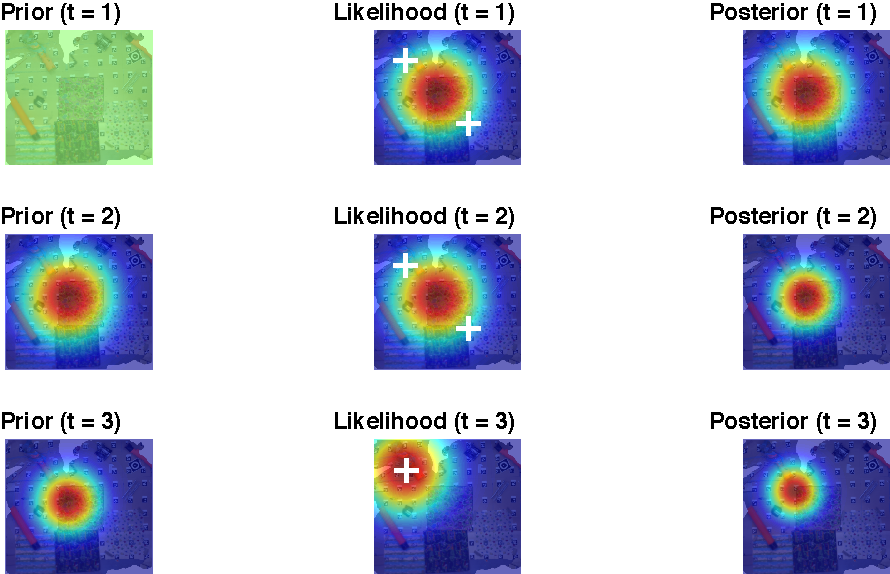
\includegraphics[width=0.7\columnwidth]{kalman-crop}
\caption[Kalman Filter.]{{\label{fig:kali} Four time steps of a Kalman
    filter for two-dimensional position estimates. The colors
    represent the probability of an $x,y$-position (red: high
    probability; blue: low probability). In timestep $t = 1$, the
    filter is initialized with an uniformed prior and each position
    has equal probability. The likelihood is calculated by the outputs
    of the $k$-NN algorithm, taking measurement error into
    account. The posterior results from the multiplication of the
    prior with the likelihood and indicates the position estimates
    after one timestep. In the next timestep, the previous posterior
    gets updates with process noise and becomes the new prior.}}
\end{center}
\end{figure}

To filter out outliers and smooth estimates, a popular filter choice
is the Kalman filter. However, the Kalman filter is not able to
represent multimodal probability distributions. This makes it rather
unsuitable for the presented approach. The naive approach in $k$-NN
regression calculates the mean of the $k$ outputs and forwards this
value to the Kalman Filter. However, if the output values are spaced
out, averaging them would yield a value in the center between them,
which is not likely to be the correct position
(Figure~\ref{fig:kali}). This approach can lead to biased
predictions, especially, if the model outputs belong to distant
locations due to similar texton distributions at these positions.

%Over time, however, the positional ambiguity, can be resolved, when
%both estimates of the $k$-NN model fall together. Compared to the
%Kalman filter, a full Bayesian filter could immediately find the
%correct position (Figure~\ref{fig:bayesianfilter}). Since a full
%Bayesian filter is computationally complex, a variant that is based on
%Monte Carlo sampling was used: the particle filter. A detailed
%description of the filtering technique can be found in the next
%section.


We decided to use a more sophisticated method to capture
\emph{multimodal distributions}.  A general Bayesian filter can
simultaneously maintain possible locations and resolve the ambiguity
as soon as one location can be favored (Figure~\ref{fig:bayes}). In
this case, the predictions of the $k$ neighbors can be directly fed
into the filter without averaging them first. The filter is able to
smooth the estimations, handle uncertainty, and simultaneously keep
track of several competing position estimations. Since a general
Bayesian filter is computationally complex, a variant that is based on
random sampling was used: the particle filter.

\begin{figure}[t]
\begin{center}
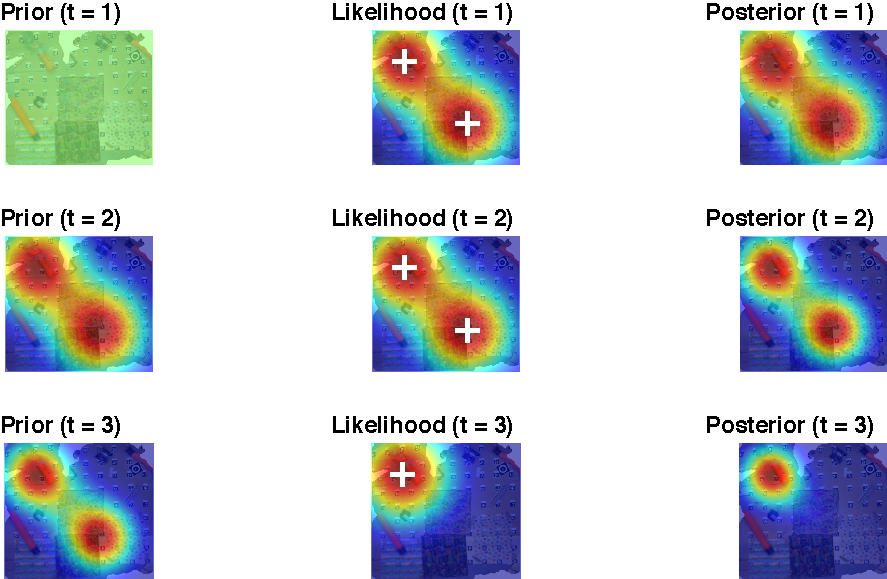
\includegraphics[width=0.7\columnwidth]{particle-crop}
\caption[Bayesian Filter.]{{\label{fig:bayes} Four time steps of a
    Bayesian filter. The colors represent the probability of an
    $x,y$-position (red: high probability; blue: low probability).}}
\end{center}
\end{figure}

The weighted particles are a discrete approximation of the posterior
probability function ($pdf$) of the state vector ($x,y$-position of
the MAV). Estimating the position of the UAV can be described as
$p(X_t \mid Z_t)$, where $X_t$ is the state vector at time $t$ and
$Z_t = \mathbf{z}_1, ..., \mathbf{z}_t$ are all outputs up to time $t$
from the $k$-NN algorithm, where each $\mathbf{z}_i$ represents the
$k$ $x,y$-outputs of the algorithm at time $i$.
% The state vector is \emph{hidden}, since the variables cannot be
% measured directly, therefore the situation can be described with a
% hidden Markov model.  Instead, noisy or ambiguous data can be
% obtained through the proposed algorithm.
The algorithm of the developed particle filter is presented in the
pseudo code in Algorithm~\ref{alg:particle_filter}, where $M$
represents the number of particles.
\begin{algorithm}
\caption{Particle filter update}
\label{alg:particle_filter}
\begin{algorithmic}[1]
  \Procedure{Particle\_Filter}{$\mathcal{X}_{t-1}, z_t$}
  \Comment $q$ is process noise, $r$ is measurement noise
  %\State $q_x^2 = 15$, $q_y^2 = 15$, $r_x^2 = 100$, $r_y^2 = 100$
  \LineComment{Particle update}
  \For{$m = 1$ to $M$}
  \LineComment{Iterate over predictions from $k$-NN}
  \For{$i = 1$ to $k$}
      % p = binormpdf(xs[i].x, xs[i].y, z[pred].x, z[pred].y,
      %               measurement_noise_x, measurement_noise_y, rho);
      % total_likelihood $\gets$ total_likelihood;
       \State sample $x_t^{[m]} \sim \mathcal{N}(x_{t-1}^{[m]}, q_x^2)$
       \EndFor
%  \State sample $y_t^{[m]} \sim \mathcal{N}(y_{t-1}^{[m]}, q_y^2)$
  \State $w_t^{[m]} \gets p(z_t^x \mid x_t^{[m]}) p(z_t^y \mid y_t^{[m]})$
  % Resampling wheel
  \EndFor
  \LineComment{Importance resampling}
  \State $\mathcal{X}_t \gets$ \Call{Resampling\_Wheel}{$\mathcal{X}_{temp}, w_t$}
  \EndProcedure
\end{algorithmic}
\end{algorithm}
The ``resampling wheel''~\cite{thrun}
(Algorithm~\ref{alg:resampling_wheel}) prevents that particles with a
low weight ``collapse''; instead, these particles are replaced by new
particles that are selected with a probability proportional to their
weight. The employed motion model is solely based on Gaussian noise
and does not consider velocity estimates are headings.
\begin{algorithm}
\caption{Resampling wheel}
\label{alg:resampling_wheel}
  \begin{algorithmic}[1]
    \Procedure{Resampling\_Wheel}{$\mathcal{X}_{temp}, w_t$}
    \State $\mathcal{X}_t \gets \emptyset$
    \State sample $\text{idx} \sim M\cdot\mathcal{U}(0, 1)$
    \State $\beta \gets 0$
    \For{$m = 1$ to $M$}
    \State $\beta \gets \beta + \mathcal{U}(0, 1)\cdot 2\cdot \max(w_t)$
    \While{$\beta > w_t[\text{idx}]$}
    \State $\beta \gets \beta - w_t[\text{idx}]$
    \State $\text{idx} \gets (\text{idx} + 1) \mod M$
    \EndWhile
    \State add $\mathcal{X}_{temp}[idx]$ to $\mathcal{X}_t$
    \EndFor
\EndProcedure
\end{algorithmic}
\end{algorithm}

Particle filters have several advantages. First, one can represent
uncertainty with the variance of the state variables of the
particles. Second, the particle filter permits \emph{sensor fusion},
and can integrate data from the inertial measurement unit (IMU) or
optical flow into the position estimation. A major disadvantage is the
rather high computational complexity. This can be circumvented by
reducing the amount of particles---trading off speed and accuracy to
adapt the computational payload to the used processor.

The used particle filter is initialized with $M = 100$ particles at
random $x, y$-positions. To incorporate the noise of the estimates of
the $k$-NN algorithm a two-dimensional Gaussian Mixture Model (GMM) was used. 
%$p(z \mid x) = \frac{p(x \mid z)p(z)}{p(x)}$ is used, where
%$\textbf{x} = ((x_1, y_1), (x_2, y_2), \ldots, (x_k, y_k))^T$. A
%a two-dimensional Gaussian sensor model was used for each resulting in
%a Gaussian Mixture Model.
The parameters of the Gaussian have been determined by comparing the
positions based on the motion tracking system with the predictions of
the texton-based system.
%(Figure~\ref{fig:measurementmodel}).
This results in values for the variances in $x$ and $y$, the
correlation $\rho$ between $x$ and $y$. The mean values $\mu$ were set
to zero (no systematic bias).

%\begin{figure}
%  \label{fig:cor_sim_confi}
%  \centering
%  \begin{subfigure}[b]{0.5\textwidth}
%  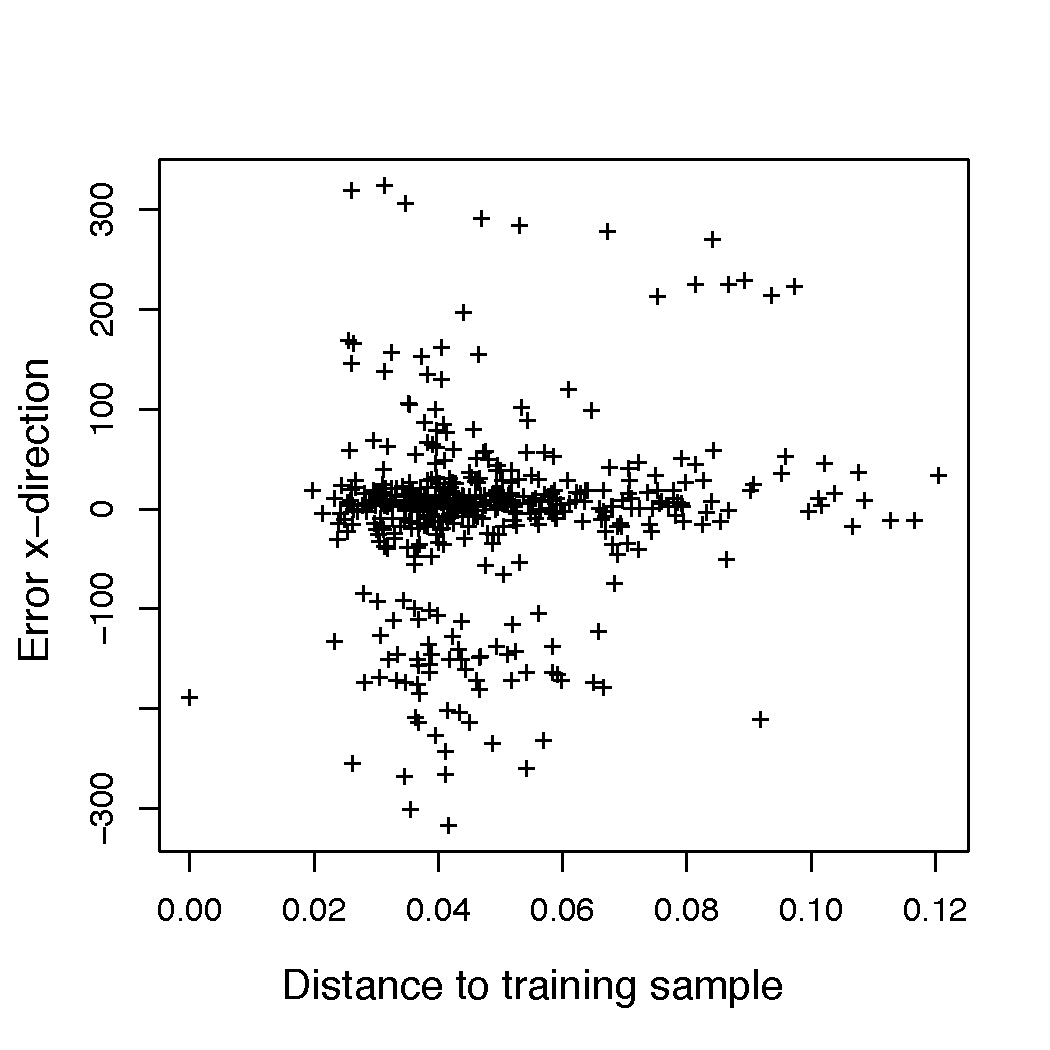
\includegraphics[width=1\textwidth]{dependency_dist_error_x}
%    %\captionof{figure}{$POS_x$}
%  \label{fig:cosinesim}
%  \end{subfigure}%
%~
%  \begin{subfigure}[b]{0.5\textwidth}
%  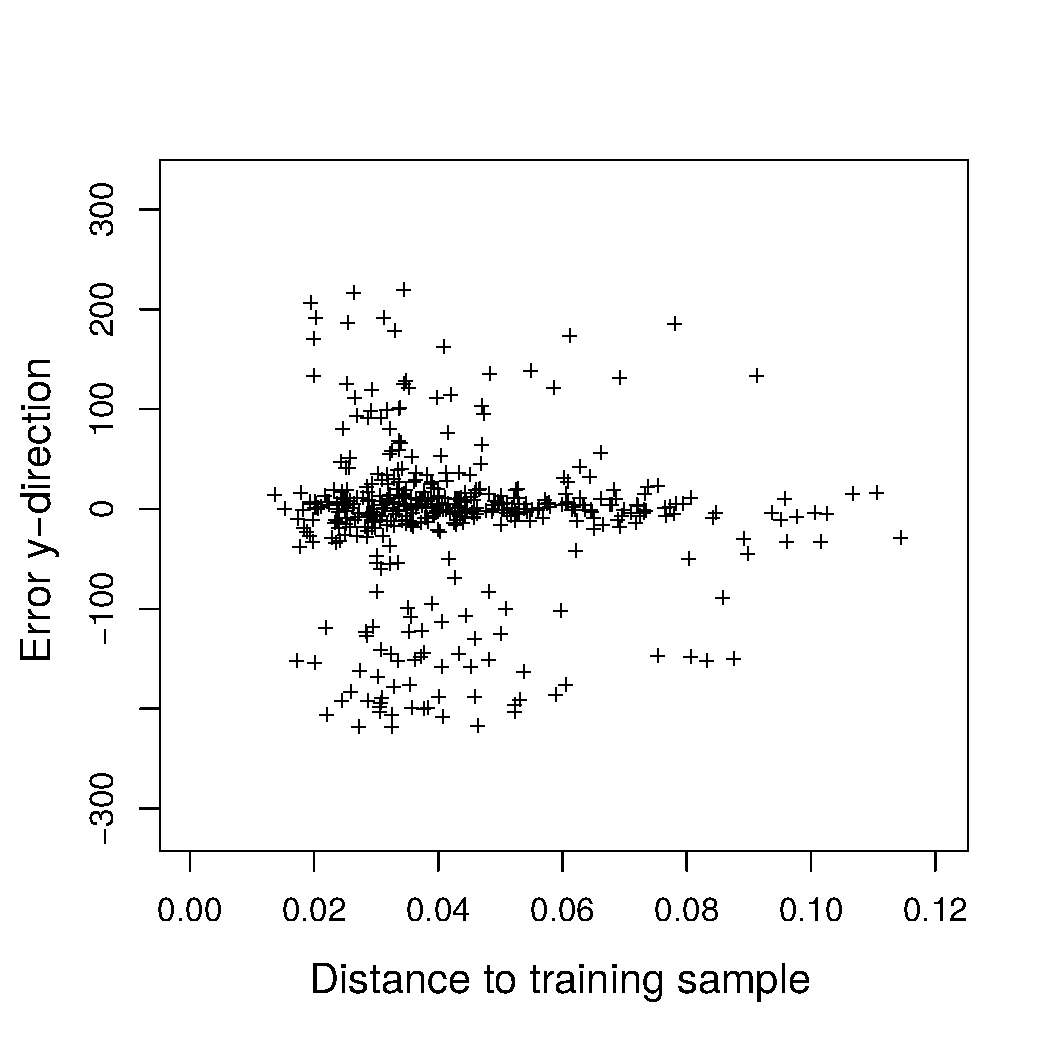
\includegraphics[width=1\textwidth]{dependency_dist_error_y}
%   % \captionof{figure}{$POS_y$}
%  \label{fig:cosinesd}
%  \end{subfigure}
%  \caption{Measurement error in $x$-direction (\emph{Left}) and
%    $y$-direction (\emph{Right}) as a function of the distance to the
%    closest training sample.}
%\label{fig:cosine}
%\end{figure}
%\unsure{uiui, should edit the labels of the y axis and uses crosses in
%both cases}
%\begin{figure}[h!]
%\label{fig:measurementmodel}
%\begin{center}
%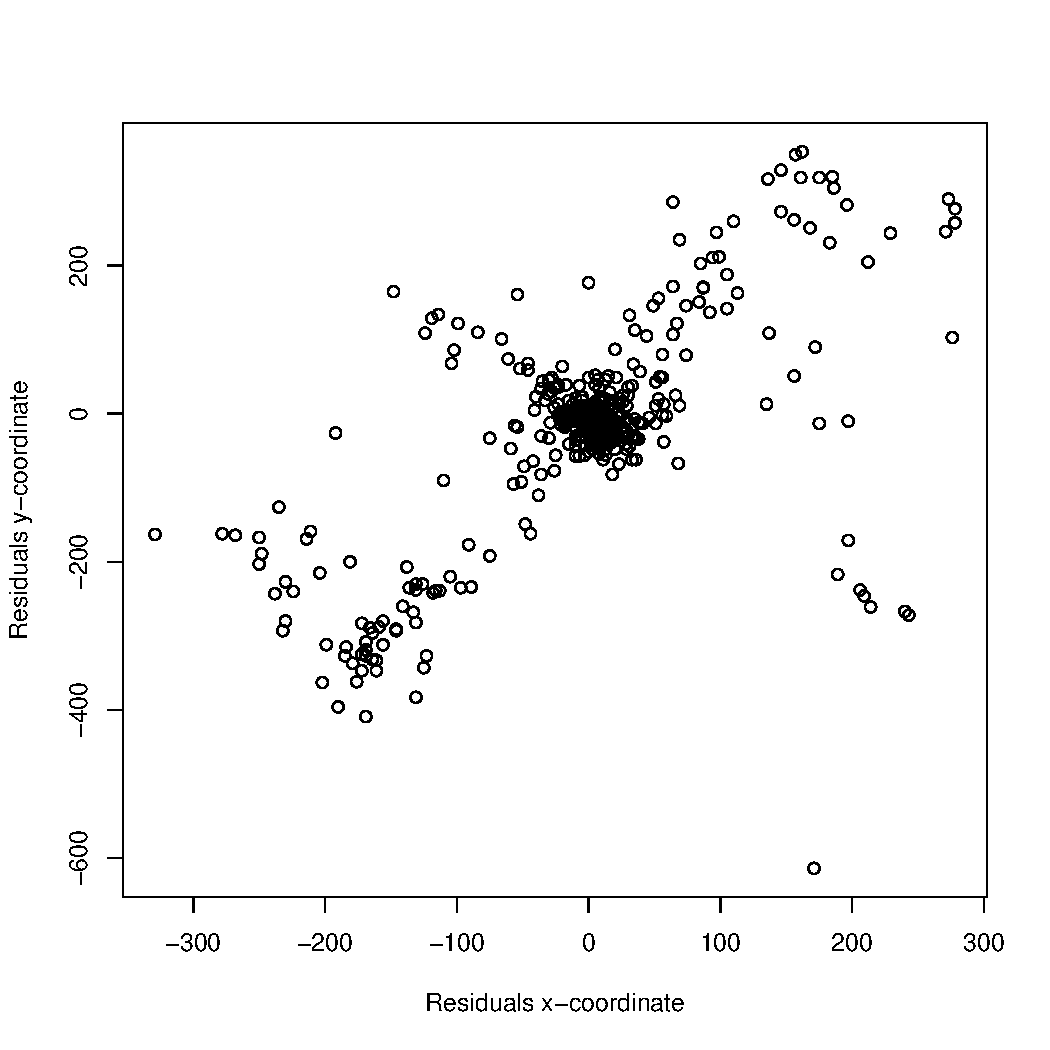
\includegraphics[width=0.448\columnwidth]{measurement_model}
%\caption{{Measurement model showing the delta x and delta y positions.
%  }}
%\end{center}
%\end{figure}
%\unsure{TODO: Add Gaussian approximation!}
The particle filter allows for using the information of all $k$
neighbors and keep track of a multimodal distribution. While keeping
track of a multimodal distribution allows for incorporating several
possible states of the system, the system needs one best position
estimate for guidance and stabilization after each iteration. Using a
weighted average of the modes would again introduce the problem that
the weighted average could fall into a low density region. Therefore,
the maximum a posteriori estimate, as described by
\citeauthor{driessen2008map} was used~\cite{driessen2008map}. This
approach uses the following formula to obtain the MAP estimate:
\begin{align}
  s_k^{MAP}  &= \text{arg}\max_{s_k}{p(s_k \mid Z_k)}\\
             &= \text{arg}\max_{s_k}{p(z_k \mid s_k) p(s_k \mid Z_{k-1})} 
\end{align}
Therefore, the final position estimate is equal to the position of one
of the particles. The MAP estimator in our case is
\begin{align}
s_k^{MAP} = \text{arg}\max_{s_k} \lambda^M(s_k)
\end{align}
with
\begin{align}
\lambda^M(s_k) = p(z_k \mid s_k) \sum_{j=1}^Mp(s_k \mid s_{k-1}^j)w^j_{k-1}
\end{align}
This function is now only evaluated at a finite, chosen number of
states, the particles, using
\begin{align}
\hat{s}_k^{MAP} = \text{arg}\_{s_k \in \{s_k^i \mid i=1,\ldots,N\}} \lambda^M(s_k)
\end{align}
In this formula, $p(z_k \mid s_k)$ is the likelihood of the particle
$s_k$ given the current measurement $z_k$. In our setting, this
probability is equal to the weight of the particle $z_k$, therefore
$p(z_k \mid s_k) = w^i_k$.

The estimation of \emph{uncertainty} is a core part of the proposed
approach, due to its importance for safety and accuracy. Therefore,
uncertainty was modeled using the spread of the particles---as
expressed by their variance in $x$-direction and $y$-direction.
%These estimates are noisy, as illustrated
%in Figure~\unsure{TODO: add edgeflow noisea add fig:edgeflow}:
%Optical flow estimates accumulate errors over time. 
%the outputs of the $k$-NN algorithm are independent of previous
%predictions. Therefore, the predictions could `jump' to locations due
%to prediction errors. The particle filter is used to combine the
%advantages of both methods and eliminate the disadvantages.
Initially, we planned to include the similarity between the current
histograms and each of the $k$ neighbors as confidence value, thus
reducing the measurement noise if a high similarity between current
histogram and a training histogram is achieved. However, we found no
correlation between these variables.
% (Figure~\ref{fig:cor_sim_confi})
We also tried to use the amount of detected keypoints ($K$) as
confidence value for the quality of the sample in the training set if
the homography-based approach is used for labeling. Again, no linear
relationship between $K$ and the error in $x$-direction ($X$) and the
error in $y$-direction ($Y$) could be found
%(Figure~\ref{fig:cor_keypoints})
: $\rho_{K, X} = 0.10$,
$\rho_{K, Y} = 0.01$.

%\begin{figure}
%  \label{fig:cor_keypoints}
%  \centering
%  \begin{subfigure}[b]{0.5\textwidth}
%  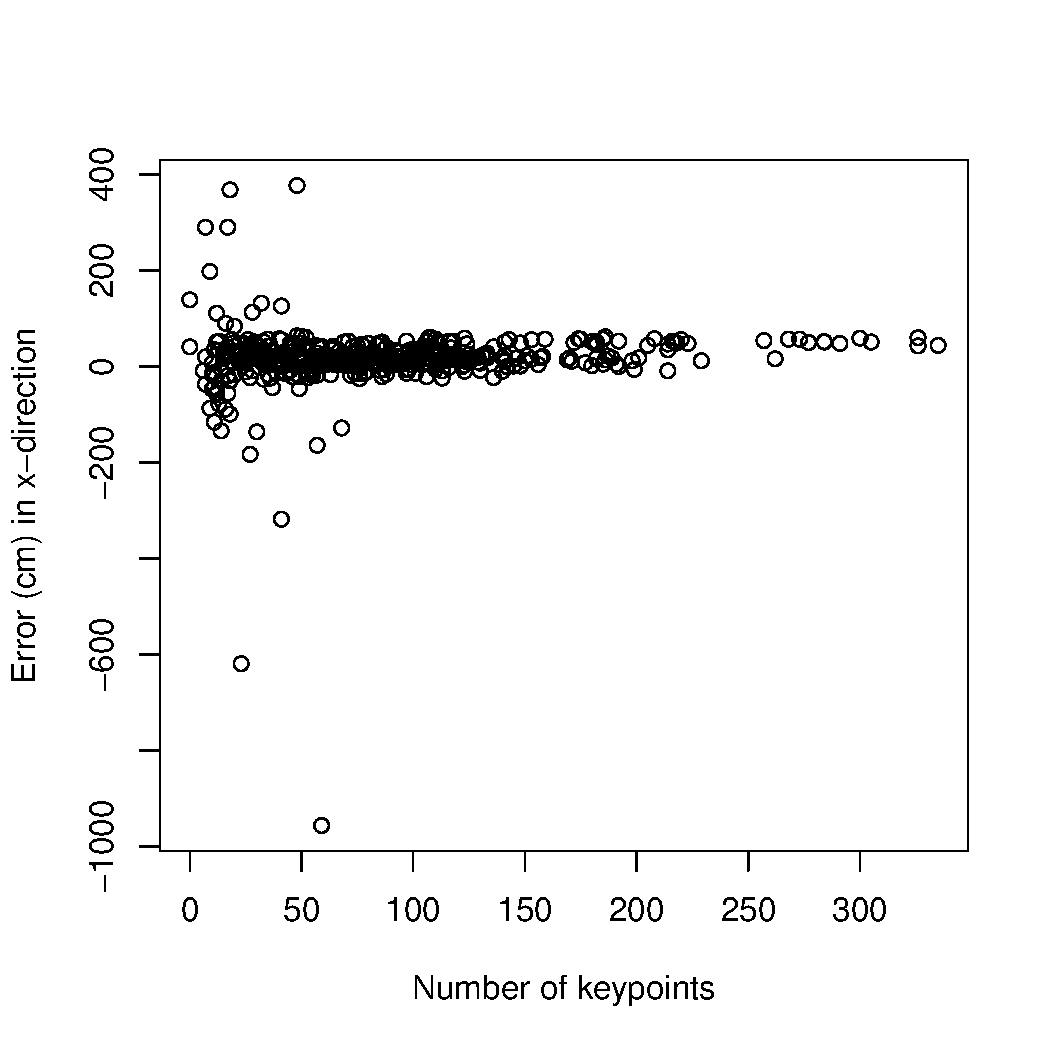
\includegraphics[width=1\textwidth]{keypoints_error_x1}
%    %\captionof{figure}{$POS_x$}
%  \label{fig:cosinesim}
%  \end{subfigure}%
%~
%  \begin{subfigure}[b]{0.5\textwidth}
%  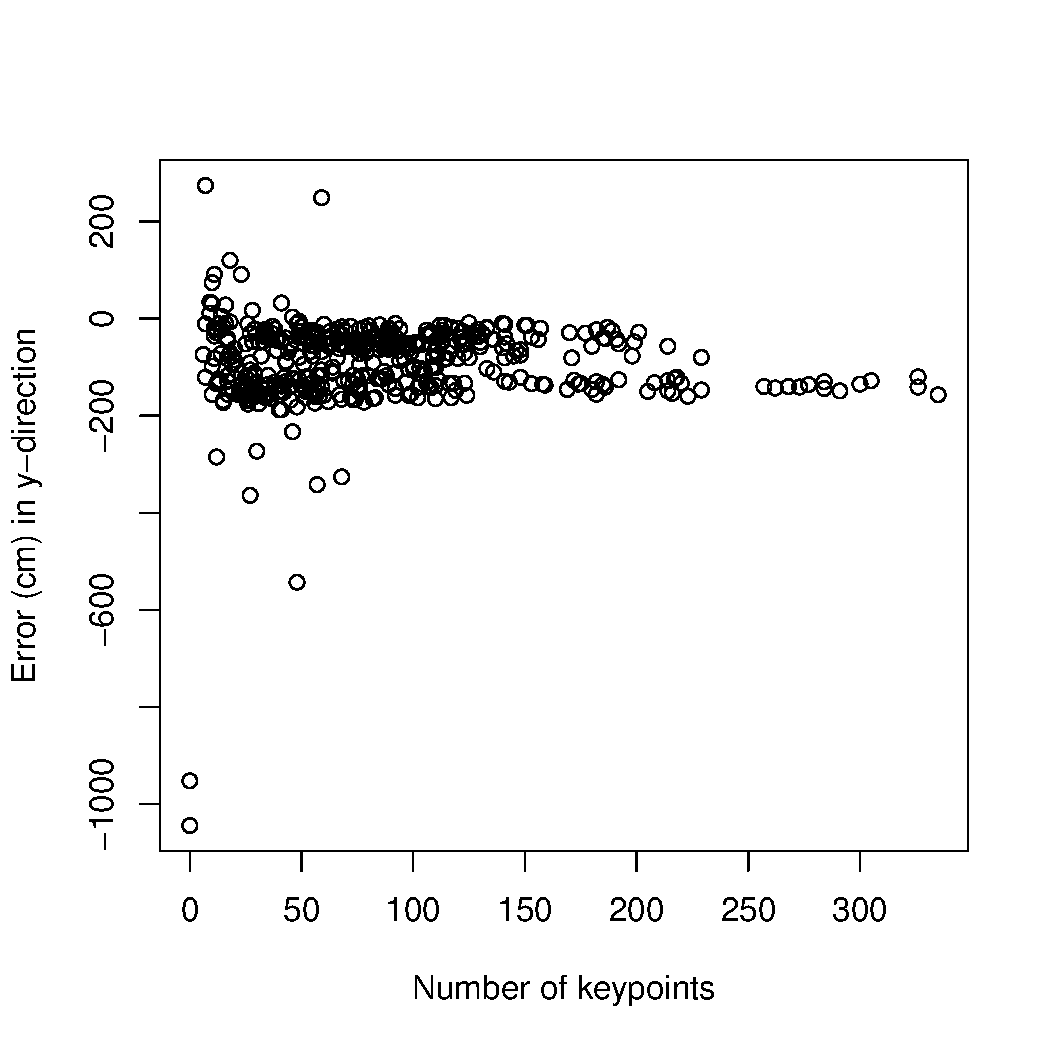
\includegraphics[width=1\textwidth]{keypoints_error_y}
%   % \captionof{figure}{$POS_y$}
%  \label{fig:cosinesd}
%  \end{subfigure}
%  \caption{Measurement error in $x$-direction (\emph{Left}) and
%    $y$-direction (\emph{Right}) as a function of the number of
%    keypoints found by \textsc{Sift}.}
%\label{fig:cosine}
%\end{figure}
%
%\unsure{uiui, should edit the labels of the y axis and uses crosses in
%both cases}
%\begin{figure}[h!]
%\label{fig:measurementmodel}
%\begin{center}
%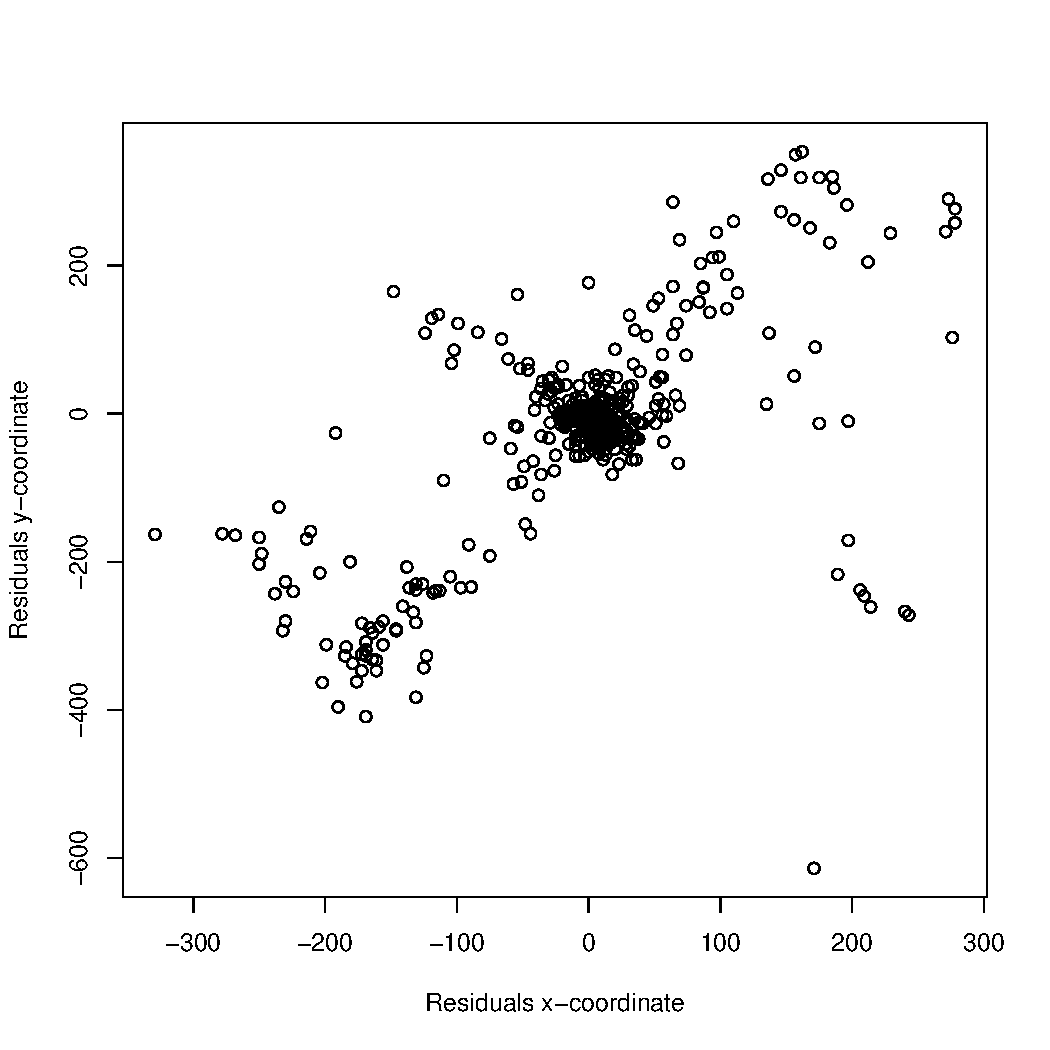
\includegraphics[width=0.448\columnwidth]{measurement_model}
%\caption{{Dependence between number of keypoints and error in
%    $x$-direction (\emph{Left}) and $y$-direction (\emph{Left}).%
%  }}
%\end{center}
%\end{figure}
%

\section{Pillar III: Map evaluation}
\label{sec:mapeval}

\subsection{Synthetic Data Generation}
\label{sec:syntheticdatageneration}

In the scope of this thesis, an application to simulate different
camera positions during flight was created. It generates synthetic
image patches based on perspective transformations of a map
image. Examples of generated images are displayed in
Figure~\ref{fig:montage}. The application allows for comparing and
predicting the performance of different maps. The software is written
in C++ and OpenCV~3.0.0.  It generates a specified amount of image
patches using random values for rotational angles, translational
shifts, as well as blur, contrast, and brightness intensity. The
values are sampled from different probability distributions
(Table~\ref{tab:distributions}).

To simulate camera movements in 3D space, a 2D to 3D projection of the
image is performed first. Then, by building separate rotation matrices
$R_x$, $R_y$, and $R_z$ around the axes $x$, $y$, and $z$, the
rotations can be performed separately. Next the rotation matrix $R$ is
created by multiplying the separate matrices, i.e.,
$R = R_x \times R_y \times R_z$. The 3D translation matrix is
multiplied by the transposed rotation matrix. This step is crucial to
ensure rotation of the \emph{camera model} and not the image
itself. Finally, after performing all steps, a projection from 3D
space to 2D is applied, to obtain the transformed image.

\begin{table}[h!]
  \centering
  \begin{tabular}{llllll}
    \toprule
    \multicolumn{6}{c}{Distribution}                                                         \\
    \multicolumn{3}{c}{Uniform ($\mathcal{U}$)} & \multicolumn{3}{c}{Normal ($\mathcal{N}$)} \\
    \cmidrule(r){1-3}\cmidrule(r){4-6}
    Parameter                                   & Min   & Max    & Parameter & M    & STD    \\
    \cmidrule(r){1-3}\cmidrule(r){4-6}
    Yaw                                         & $88$  & $92$   & Roll      & $90$ & $3$    \\
    Translation X                               & $100$ & $1800$ & Pitch     & $90$ & $4$    \\
    Translation Y                               & $100$ & $$     &           &      &        \\
    Height                                      & $190$ & $210$  &           &      &        \\
    Blurring kernel size (box filter)           & $0$   & $2$    &           &      &        \\
    Brightness                                  & $0$   & $2$    &           &      &        \\
    \bottomrule
  \end{tabular}
  \caption[Distributions for the different
  parameters of the synthetic data augmentation tool.]{The table shows the used distributions for the different
    parameters of the synthetic data augmentation tool. The values for
  blur normalized box filter and contrast }
  \label{tab:distributions}

\end{table}

\begin{figure}[h!]
\begin{center}
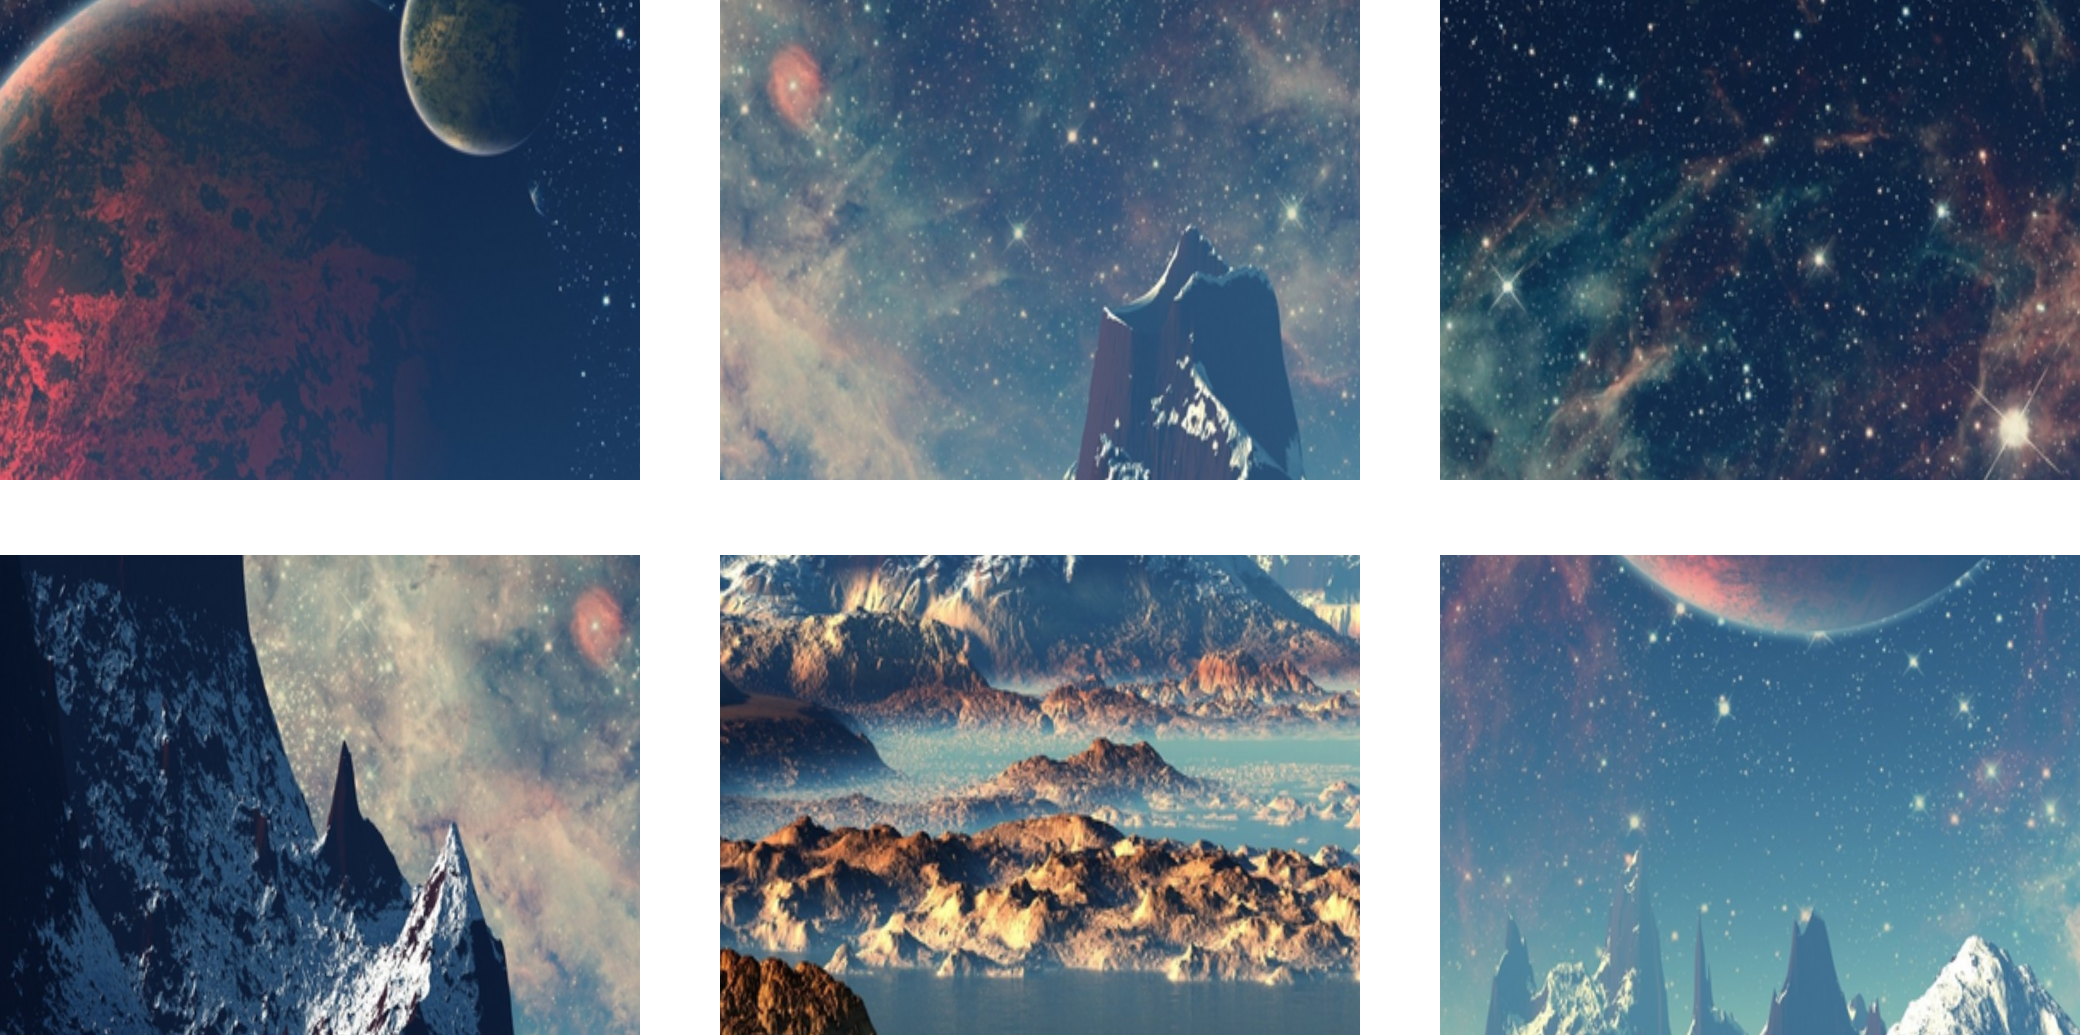
\includegraphics[width=0.7\columnwidth]{samples}
\caption{{\label{fig:montage} 
Six images generated by the synthetic data generation tool.%
}}
\end{center}
\end{figure}

\begin{figure}[h!]
\begin{center}
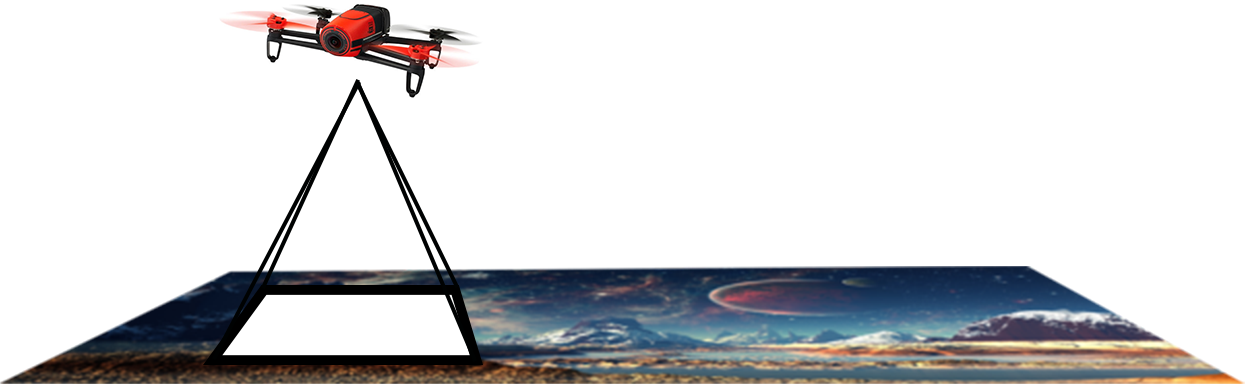
\includegraphics[width=0.672\columnwidth]{camera_model}
\caption{{Camera model for the synthetic flight.%
}}
\end{center}
\end{figure}

\subsection{Evaluation Scheme}
\label{sec:evaluationscheme}

The performance of the proposed method depends on the environment: a
texture-rich environment without repeating patterns will be better
suited than a texture-poor environment. Ideally, one would like to
know if the proposed method is able to work in a given
environment. Therefore, we propose an evaluation scheme for maps. This
scheme assigns a global fitness value to a given map, proportional to
the accuracy it is expected to achieve in the physical world. The
evaluation scheme allows to inspect the given map and to detect
regions that are responsible for the overall fitness value. The
evaluation of a map is difficult, since the obtained histograms during
a real flight depend on many factors: motion blur, distance to the map
and rotations proportional to the map.

In the first step of the map evaluation procedure, $N$ different
patches of a given map are generated using the synthetic data
generation tool (Section~\ref{sec:syntheticdatageneration}). We
propose the following global loss function ($L$) for evaluating a
given map ($\mathcal{M}$):
\begin{align}
  L(\mathcal{M}) &= \sum_{i = 1}^{N} \sum_{j = 1}^{N} \ell(d_a(h_i, h_j), d_e(h_i, h_j))
\end{align}
\begin{align}
  \ell(x, y) &= x - y\\
  d_a(h_i, h_j) &= \text{CS}(h_i, h_j)\\
  d_e(h_i, h_j) &= f_X(pos_i \mid \mu, \Sigma) = f_X(x_i, y_i \mid \mu, \Sigma)\\
\end{align}
\begin{align}
\mu = pos_j = (x_j, y_j)\\
\Sigma =
  \begin{bmatrix}
    \rho & 0\\
    0 & \rho\\
  \end{bmatrix}
\end{align}
The cosine similarity (CS) is:
\begin{align}
CS(h_i, h_j) = \frac{h_i^Th_j}{||h_i||\,||h_j||}
\end{align}
The cosine similarity has the convenient property that its values are
bounded between $-1$ and $1$. In the present case, since the elements
of $h_i$ and $h_j$ are non-negative, it is even bounded between $0$
and $1$. The function $f_x$ describes the non-normalized probability
density function of the normal distribution:
$f_X(x) = e^{- \frac{(x - \mu)^2}{2 \sigma ^ 2}}$. This function is
also bounded between $0$ and $1$, which makes the functions $f_X$ and
$CS$ easily comparable.

The idea behind the global loss function $L$ is that histograms in
closeby areas should be similar and the similarity should decrease the
further apart two positions are. This is modeled as a 2-dimensional
Gaussian with zero covariance. The variance is dependent on the
desired accuracy ($\rho$): the lower the variance, the more punctuated
a certain location is but also the higher the risk that a totally
wrong measurement occurs.

In future research, the ``bad regions'' could be optimized using an
optimization approach such as an evolutionary algorithm. It also
allows to show the similarities for a fixed position and the loss for
a fixed positions based on the expected similarity and the actual
similarity.

\begin{figure}[h!]
\begin{center}
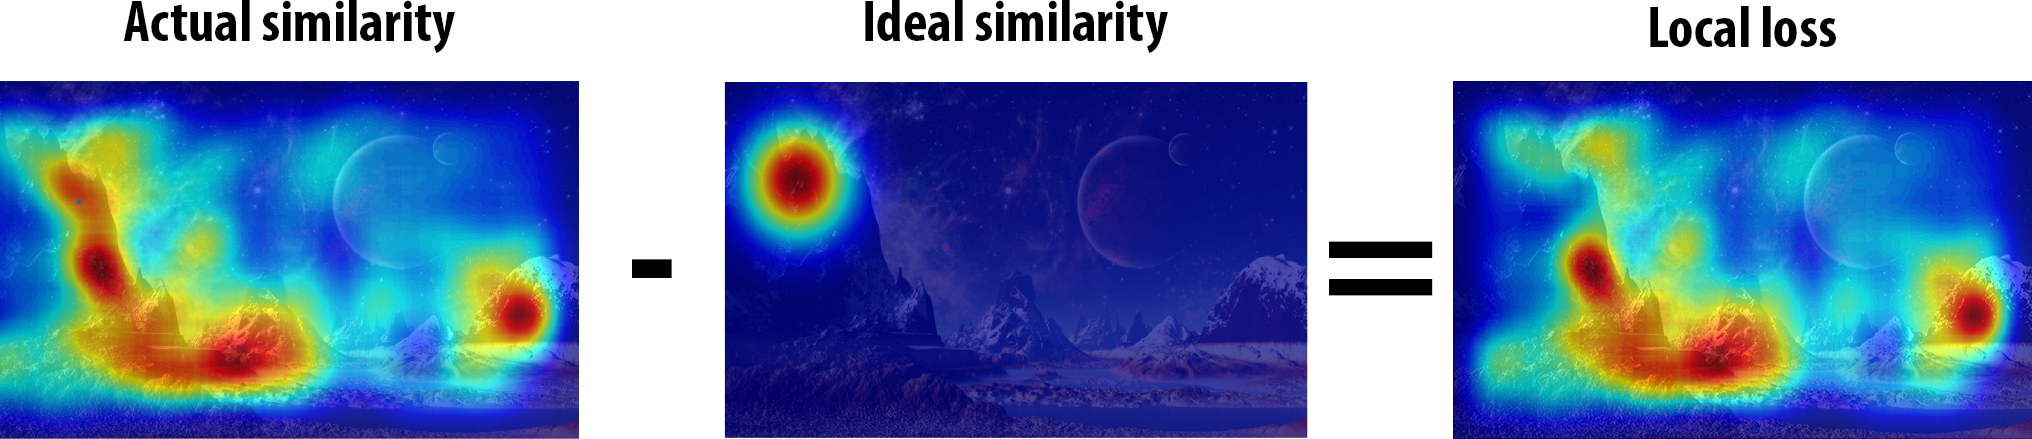
\includegraphics[width=1\columnwidth]{local_loss}
\caption{{Heatmap colors show losses per region (smoothed using a
    Gaussian filter). Ideal histogram similarity for a given
    position. Histograms taken at positions close to
    $\textbf{x} = (400, 300)$ should be similar to this histogram. The
    further away the position of a certain histogram, the lower the
    ideal similarity should be.%
  }}
\end{center}
\end{figure}

\chapter{Analysis}
\label{chap:analysis}
\unsure{Also show how the accuracy changes by introducing more textons}

In this chapter, the setup of the conducted experiments is
presented. We examine different parameter choices in Experiment~1 to 6
in on-ground experiments using recorded data. Afterward, the found
parameters are used to show the validity during flight in
Experiments~7 and 8. The experiments were conducted in TU Delft's
indoor flight arena, the ``CyberZoo.''
%(Figure~\ref{fig:cyberzoo}).
%The
%arena has relatively constant lighting settings due to primarily
%artificial lighting.
%\begin{figure}[t]
%  \centering
% 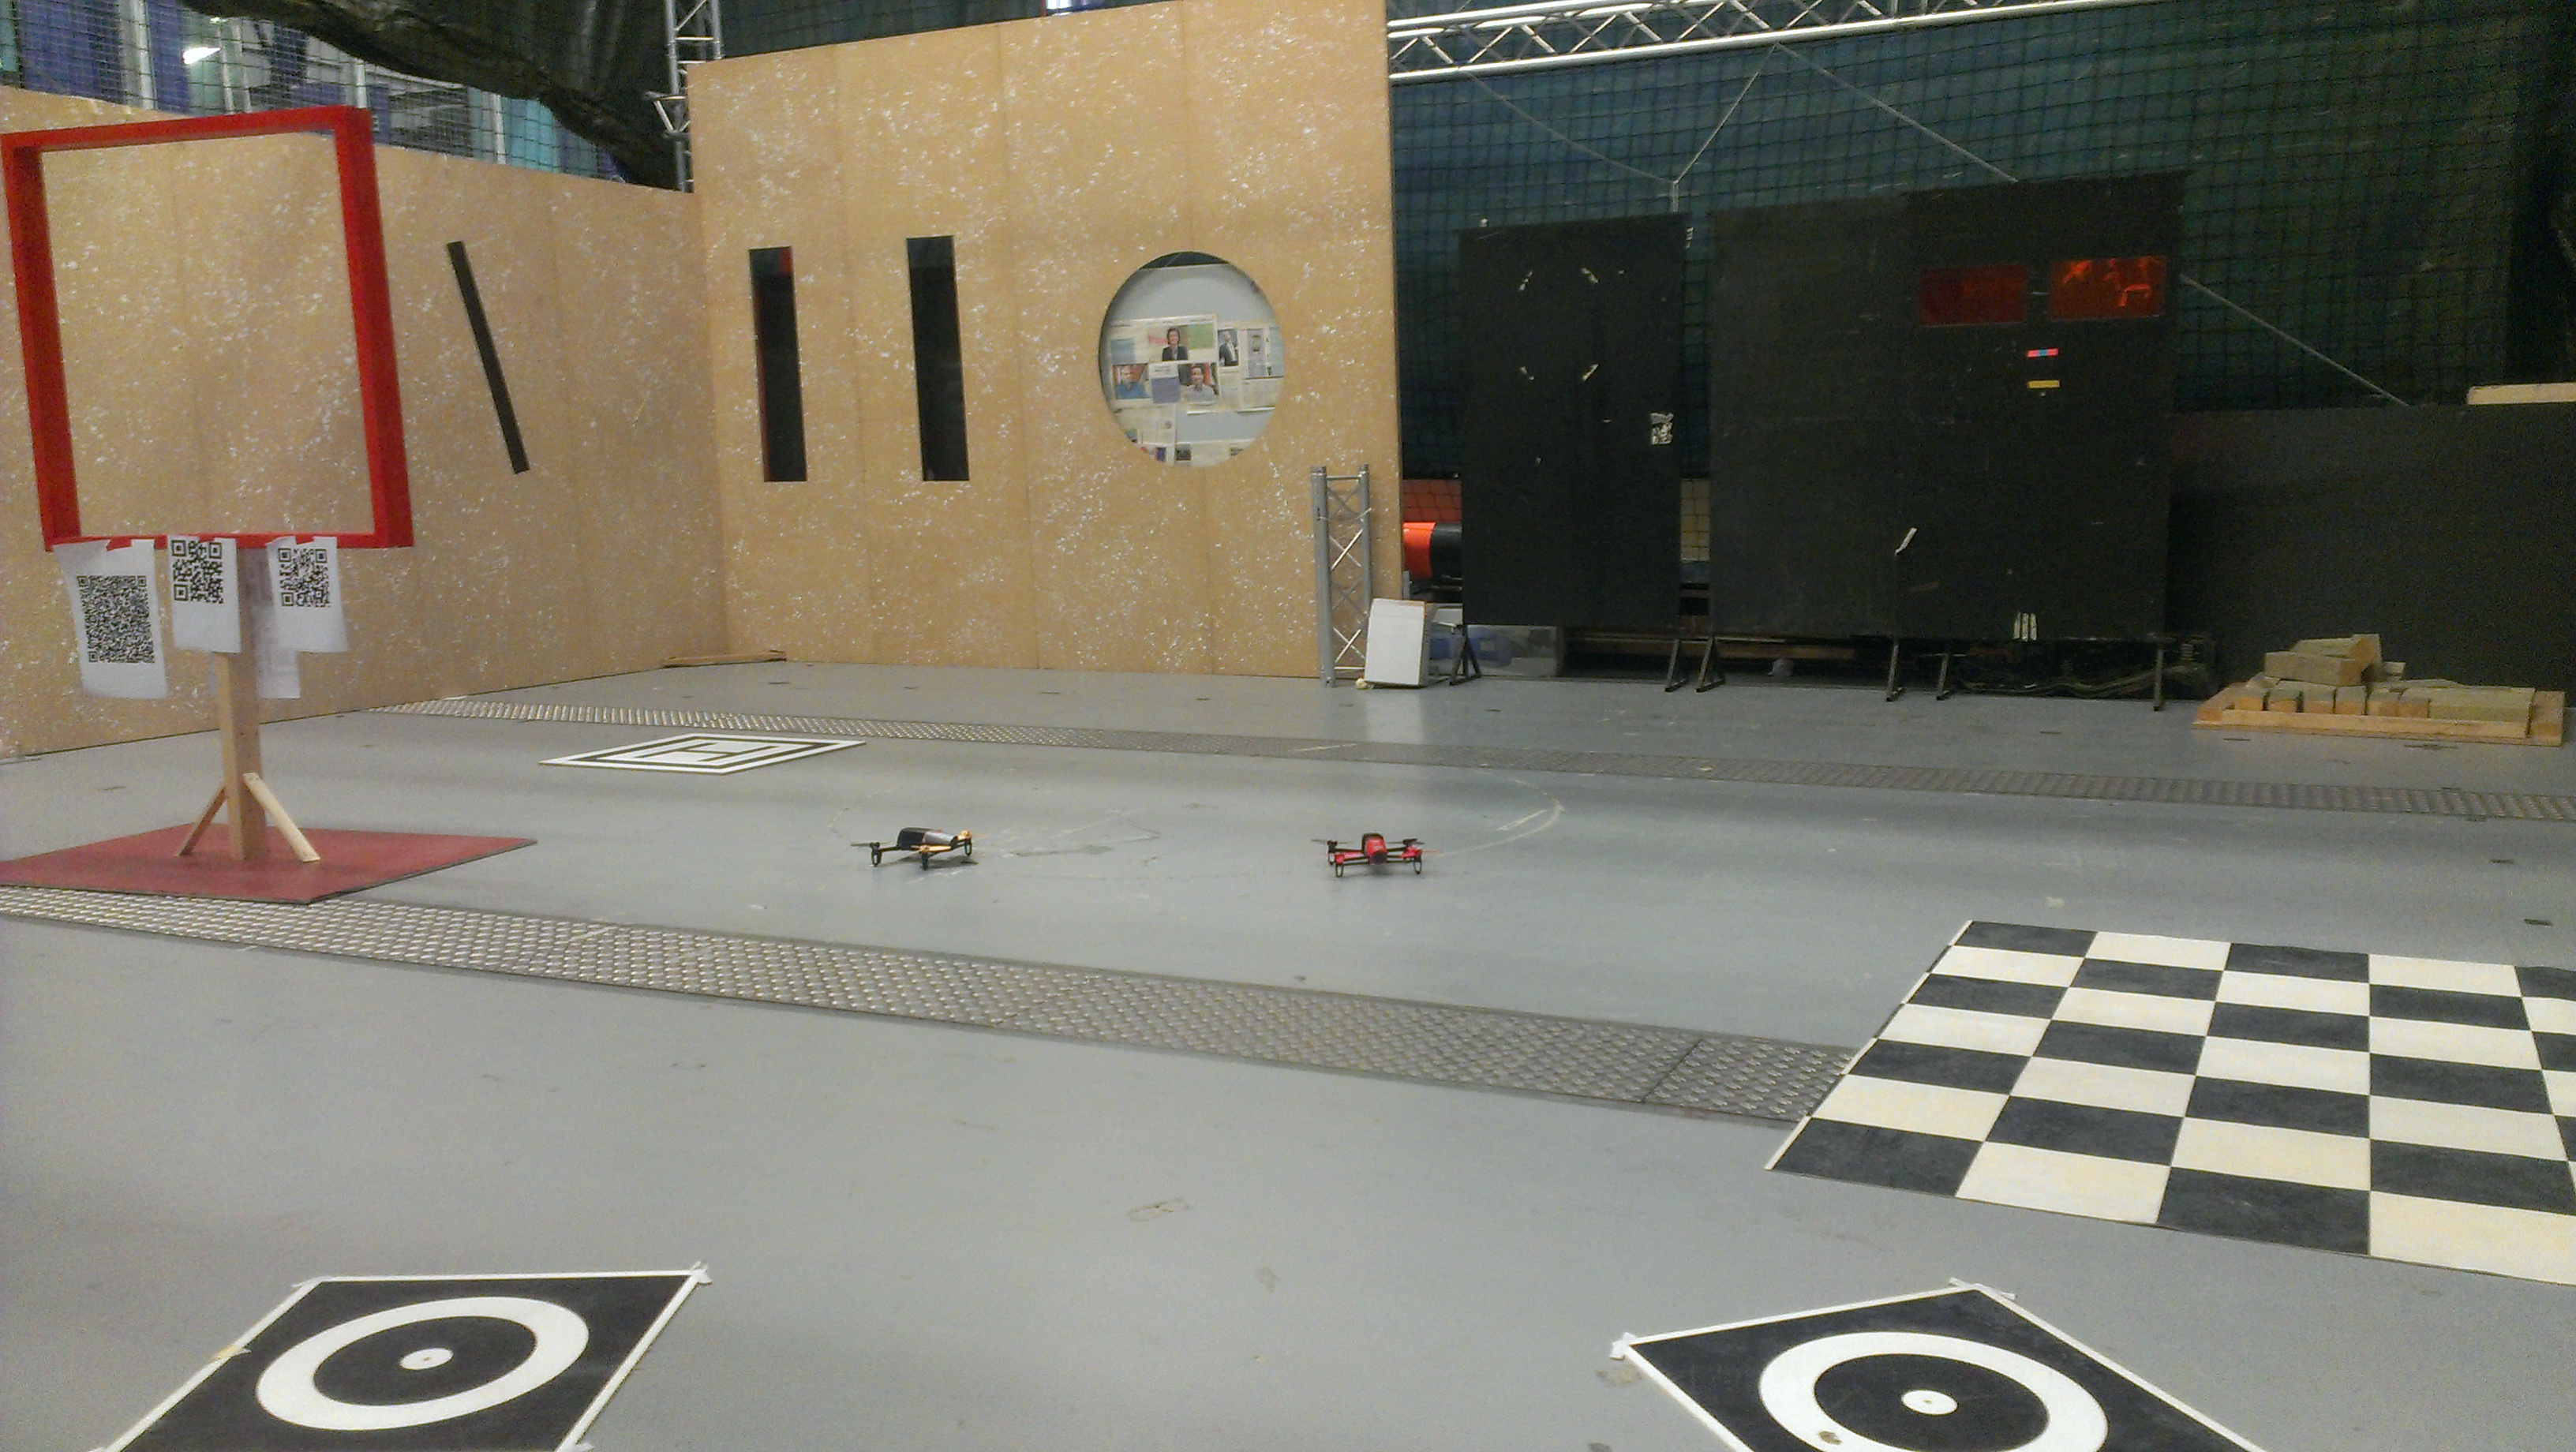
\includegraphics{cyberzoo} 
%  \caption{The indoor flight arena at the TU Delft: the ``CyberZoo.''
%  }
%    \label{fig:cyberzoo}
%\end{figure}
%
There are no generally optimal parameters for the presented framework:
Setting the number of textons, the number of images patches, or the
number of neighbors is dependent on the environment and the size of the
training dataset. The parameters have to be adapted to the particular
environment.
%since the proposed algorithm is intended for known
%environments, this is always possible.

\section{Analysis -- Determining the Number of Image Patches}
\label{sec:numtextons}

The developed framework modifies it computational complexity by
changing the number of extracted image samples. To increase the speed
of the algorithm, the goal is to use as few samples as possible. To
determine a suitable number of extracted samples, in this experiment,
the average cosine similarity between $D = 20$ datasets of histograms
is compared. Each dataset consists of $N = 10300$ histograms. The
independent variable is the number of extracted image patches $M$. The
histograms were generated using the same images. Due to the random
sampling of the extracted image patches, the histograms of each
datasets will differ. This deviation will be measured using the cosine
similarity. Therefore, each of the $D$ datasets was compared to all
the other $D - 10$ datasets and the average cosine similarity was
determined as well as the standard deviation of the cosine similarity
was measured. Comparing the cosine similarity between the histograms
has the advantage that the number of samples can be determined
independent of a specific task.

Figure~\ref{fig:cosine} displays the cosine similarity of histograms
as a function of the number of samples and the corresponding standard
deviations.

\begin{figure}[h!]
\begin{center}
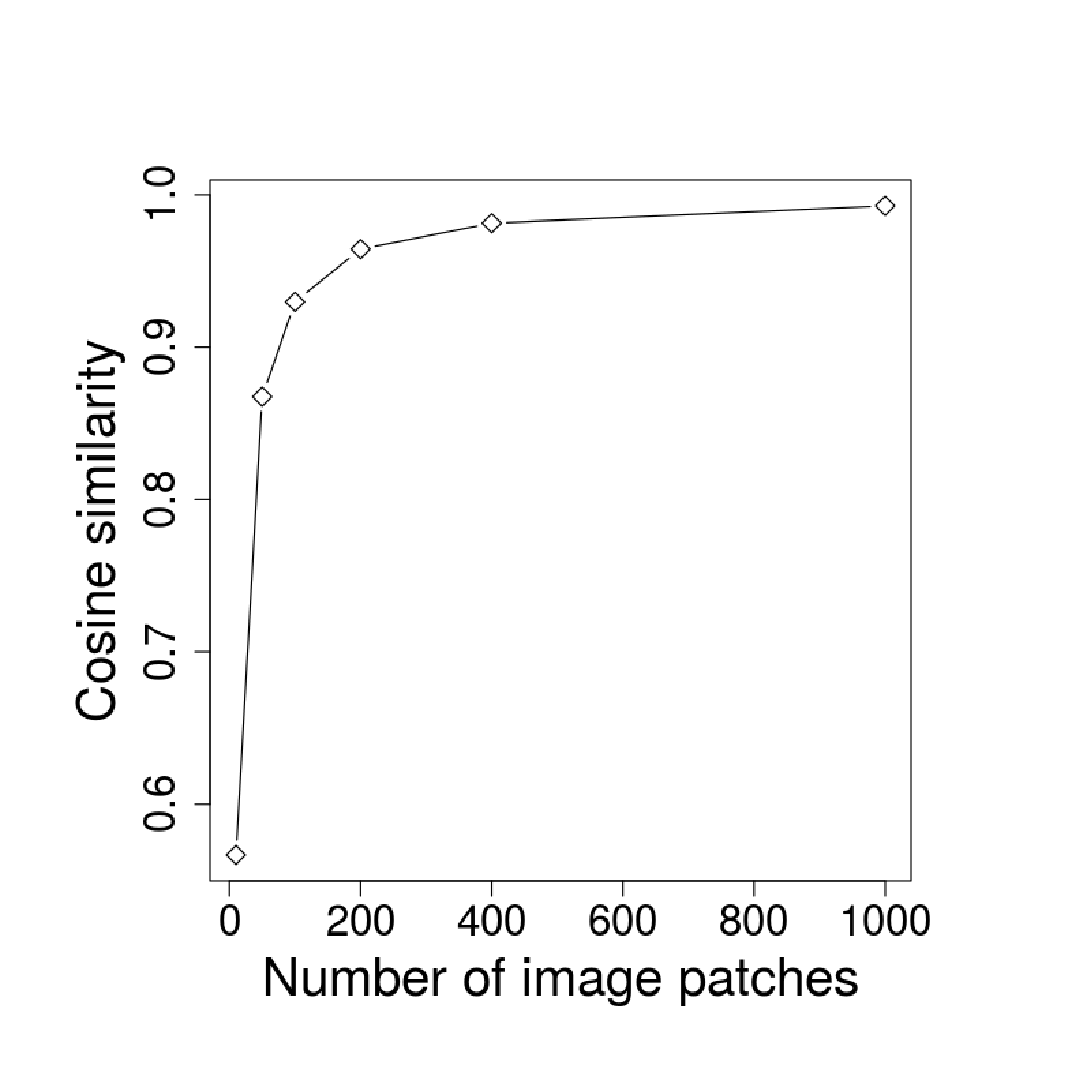
\includegraphics[width=0.336\columnwidth]{samples_vs_similarity}
\caption{{\label{fig:cosine} Cosine similarity of histograms as a
    function of the number of samples \emph{Right}: Standard deviation
    of cosine similarity in relation to the number of samples. The
    squares indicate the positions at which the dependency was
    evaluated.%%
  }}
\end{center}
\end{figure}


\section{Analysis -- Setting the Baseline for $k$-NN and determining
  $k$}
\label{sec:detk}

In a standard setting, the training error $\epsilon_t$ of a
$k$=1-nearest neighbor algorithm is $\epsilon_t = 0$ because the
nearest neighbor of the sample will be the sample itself, given that
each feature vector is unique. However, in the presented framework,
the random sampling in the histogram extraction step leads to varying
histograms.

\begin{figure}[h!]
\begin{center}
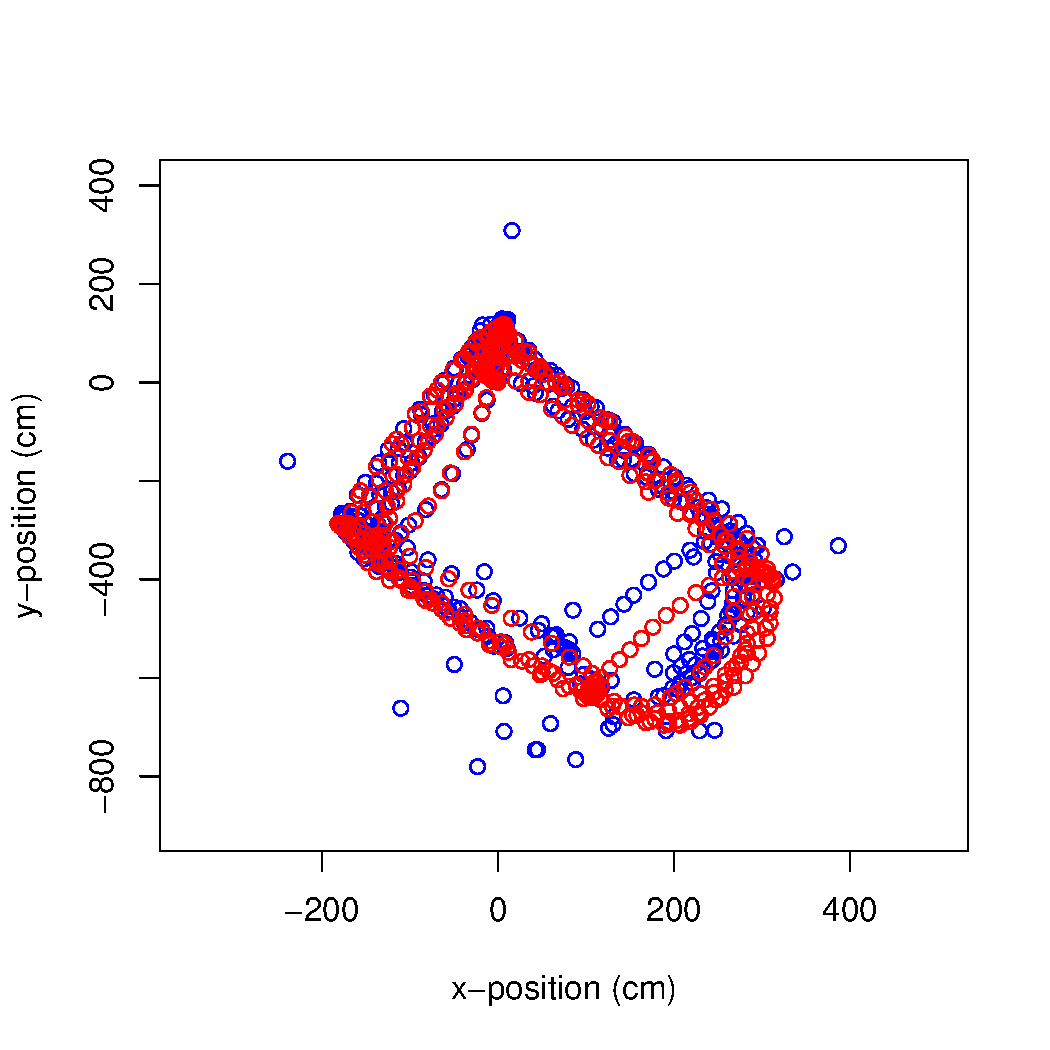
\includegraphics[width=0.448\columnwidth]{SIFT_vs_OptiTrack}
\caption{{\label{fig:flightpath} The estimates of the homography
    method compared to the ground truth of the motion tracking system.
    TODO: Legend%
  }}
\end{center}
\end{figure}

\begin{table}[H]
  \centering
  \begin{tabular}{lrrr}
    \toprule
    & x-position & y-position\\
    \midrule
    Error in $cm$ & 31 & 75\\
    STD in $cm$ & 73 & 369\\
    \bottomrule
  \end{tabular}
  \caption[Error statistics homography method.]{Error statistics for the homography method.}
  \label{tab:homoerror}
\end{table}


\section{Experiment -- Motion tracking system for Stabilization,
  Texton-based Approach for estimation}

\subsection{Training Set based on Motion Tracking System}
\label{sec:experiment-real}

In this experiment, a fixed route was set using the ground control
station. While the stabilization and guidance were performed using the
motion tracking system, the position estimates were performed on board
of the MAV using the texton-based approach. The Euclidean distances
between the estimates of the motion tracking system and the
texton-based approach were measured separately for the $x$- and
$y$-direction.  The training dataset was composed of 500 images
recorded at an height of approximately 1\,m, recorded in a time span
of one hour before the experiment. The corresponding $x,y$-coordinates
were obtained from the motion tracking system.

\begin{table}[H]
  \centering
  \begin{tabular}{lrrr}
    \toprule
    & x-position & y-position\\
    \midrule
    Error in $cm$ & 46 & 54\\
    STD in $cm$ & 56 & 71\\
    \bottomrule
  \end{tabular}
  \caption[Estimates of the texton-based approach]{Estimates of the texton-based approach}
  \label{tab:route}
\end{table}

\begin{comment}
  \begin{figure}
    \includegraphics[width=0.7\textwidth]{route}
    \caption[Estimates of the texton-based approach]{Estimates of the
      texton-based approach}
    \label{fig:route}
  \end{figure}
\end{comment}

\subsection{Training Set based on Homography-finding Method}
\label{sec:traininghomo}

In this experiment, the training dataset was created using the
homography-finding method. Apart from that, the settings are the same
as in Experiment~\ref{sec:experiment-real}.

\begin{figure}[h!]
\begin{center}
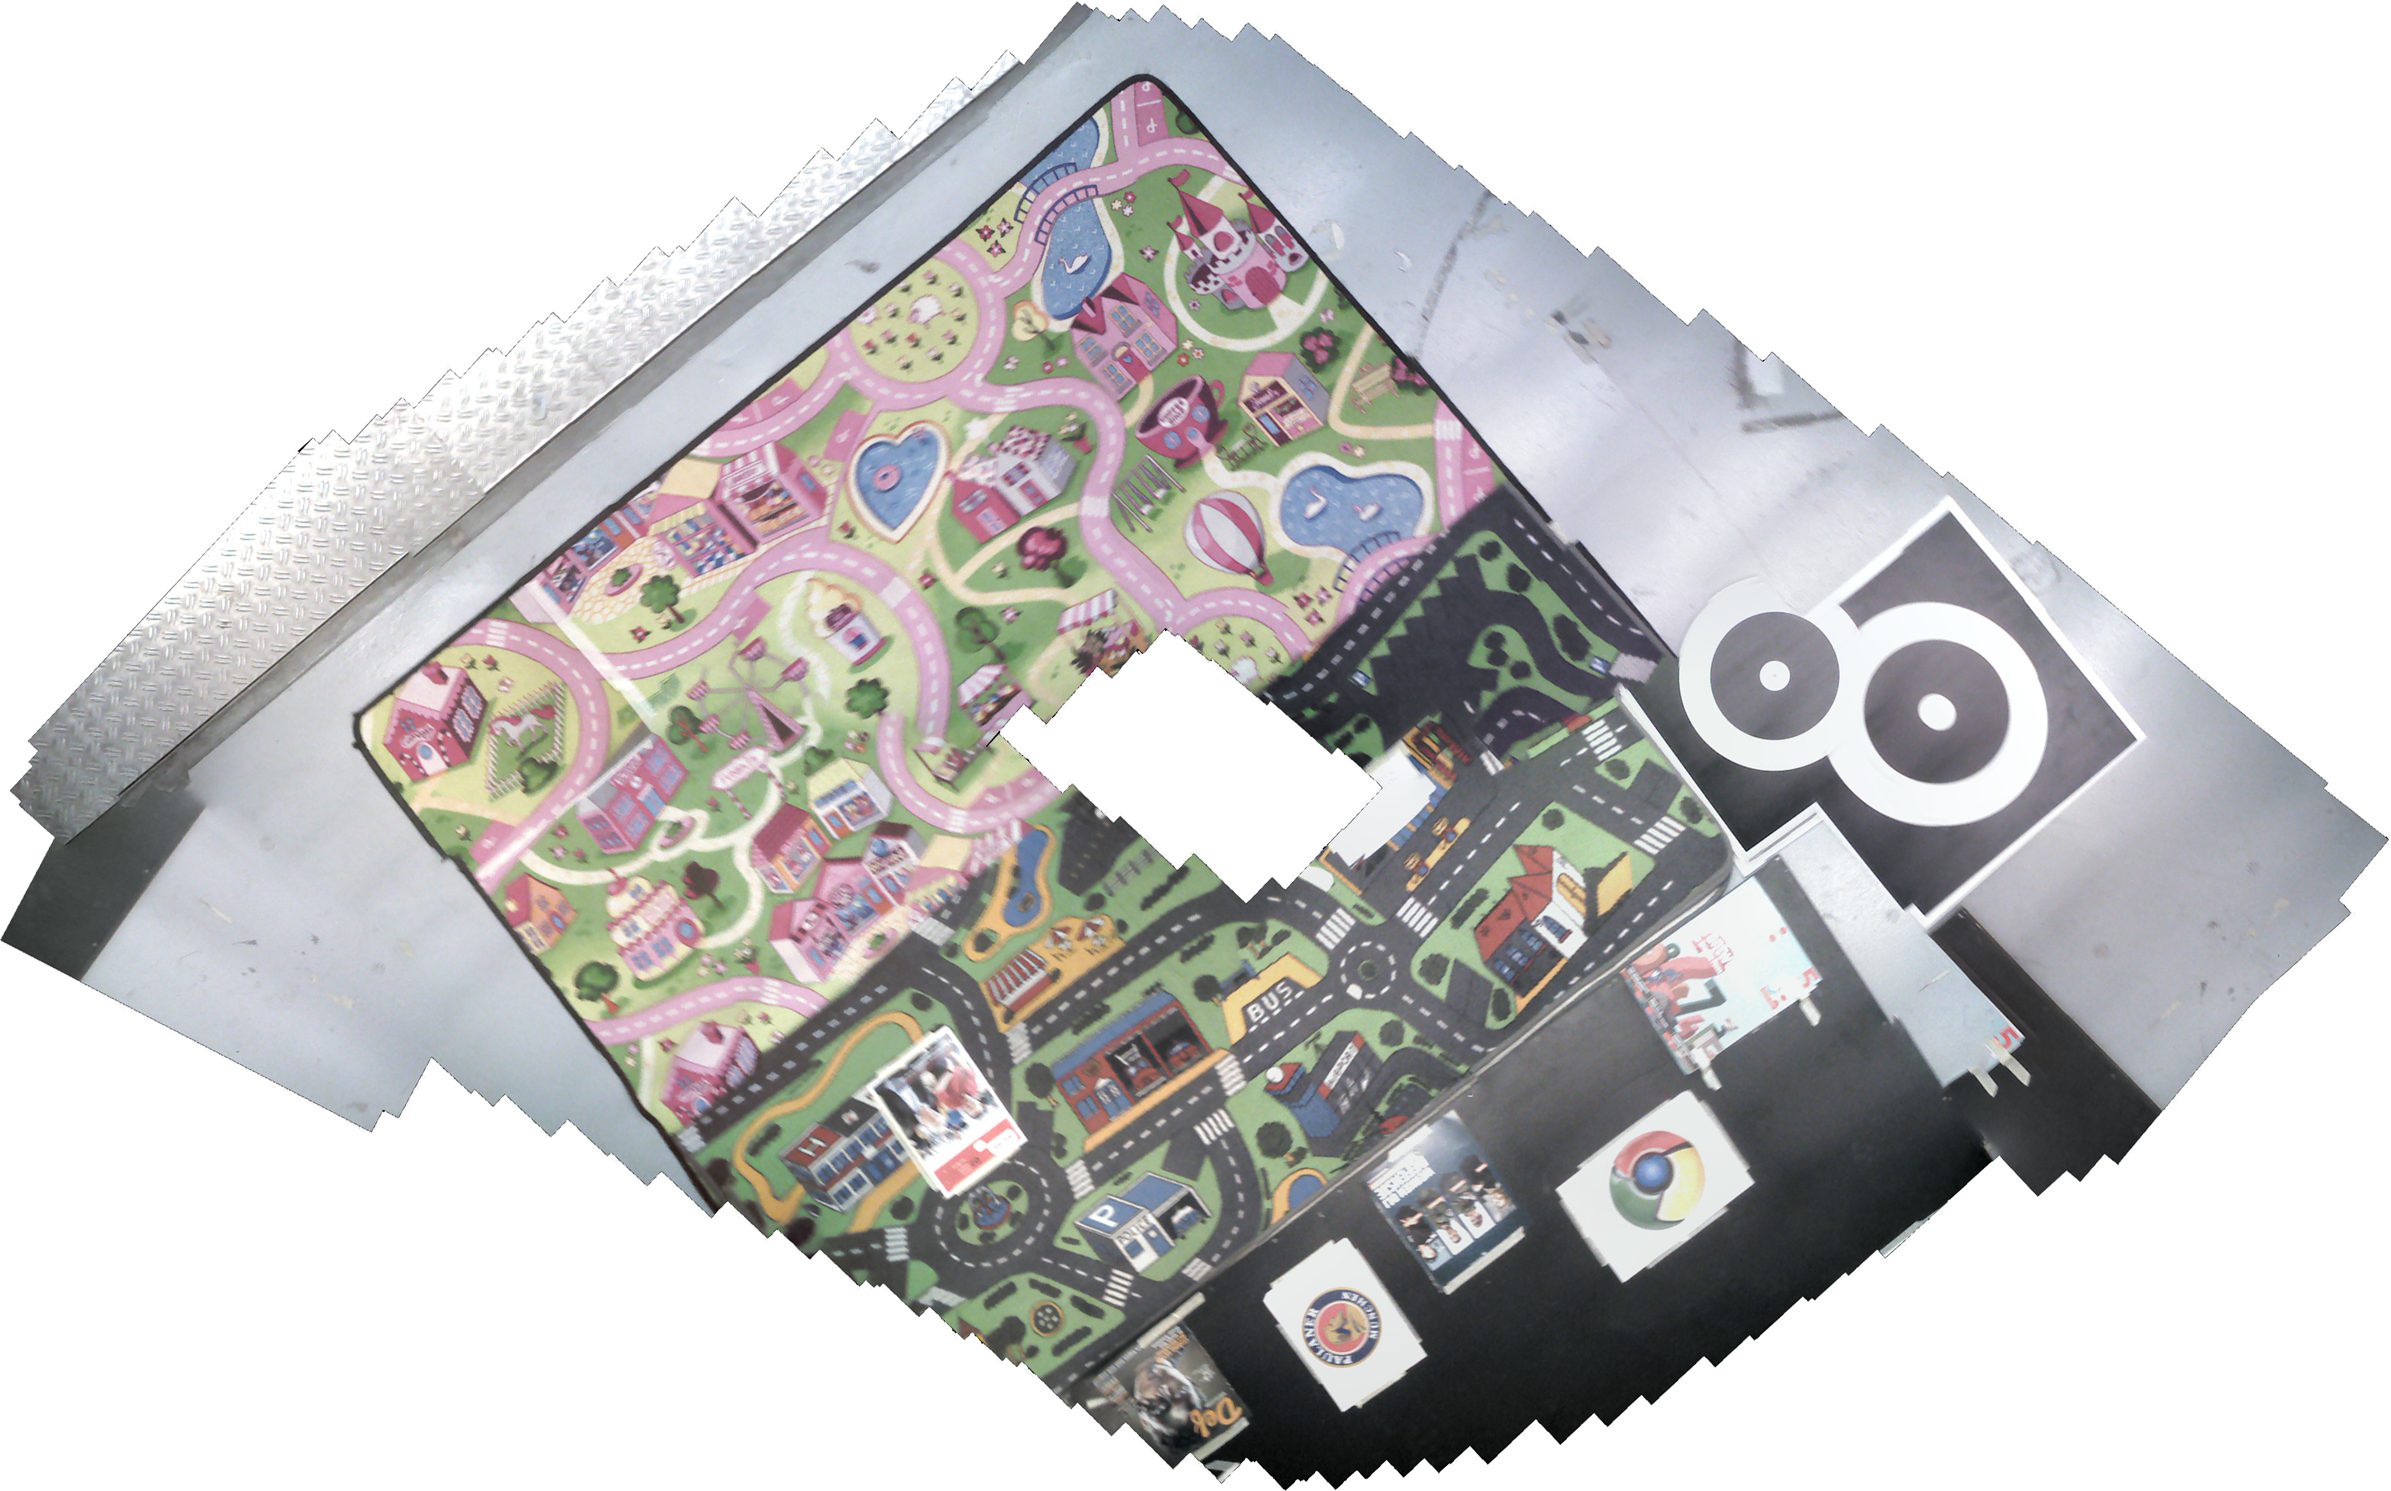
\includegraphics[width=0.7\columnwidth]{map_rotated}
\caption{{\label{fig:mapexp} The created map that was stitched
    together using 445 images. A non-mapped area in the middle of the
    map can be seen, which is a result of the set flight path. An
    image distortion can be seen at the right-hand side, where the
    landing spot sign appears twice, while in reality, only one circle
    was visible.%
  }}
\end{center}
\end{figure}


\section{Experiment -- Triggered Landing}
\label{sec:triggered}

In the triggered landing experiment, the UAV was programmed to land as
soon as its position estimates are in the landing zone. The landing
zone was defined as a circle with a radius of $60\,cm$. The
$x,y$-coordinate of the center of the circle was specified in the
flight plan. A safety criterion based on the variance of particles was
introduced, such that the landing is only performed if the criterion
holds. The criterion parameter was set to 60\,cm in both $x-$ and
$y$-direction. The experiment was conducted on a $5m \times 5m$ map
and the ground truth was based on the position data from the motion
tracking system. The training dataset was composed of 500 images
recorded at an height of approximately 1\,m, recorded in a time span
of one hour before the experiment. Table~\ref{tab:targetlanding} shows
the results of the triggered landings. Four out of six landings were
correctly performed in the landing area. The mean distance of outliers
was 16\,cm.
\begin{table}[H]
  \centering
  \begin{tabular}{lrrr}
    \toprule
    & x-position & y-position\\
    \midrule
    Error in $cm$ & TODO & TODO\\
    STD in $cm$ & TODO & TODO\\
    \bottomrule
  \end{tabular}
  \caption[Triggered landings]{Results of the triggered landings}
  \label{tab:targetlanding}

\end{table}


\section{Experiment -- Determining the Frequency}

The frequency of the proposed algorithm is determined by varying the
number of samples in the texton-based approach, the number of textons,
and the number of particles of the particle filter.

\section{Experiment -- Comparing different possible maps}

For the map comparison, 50 possible maps have been collected using the
search term `wallpaper' in Google's image search. This search term was
used, since it is (i) a general term, without any specific image
categories, (ii) wallpapers are likely to have a high resolution, and
(iii) wallpapers are likely to be visually pleasant since they are
often used as desktop backgrounds. The criteria for the images were
that their minimum resolution was $1920 \times 1080$. Images with a
higher resolution were converted to $1920 \times 1080$.  For each
image, we generated 1000 random image patches using the simulation
method described in Section~\ref{sec:syntheticdatageneration},
followed by the histogram extraction method. This yielded a labeled
dataset of histograms and corresponding positions. For each map, we
determined the expected overall loss based on the method described in
Section~\ref{sec:syntheticdatageneration}. The compared maps were then
sorted according to their estimated loss.

%Three of the compared maps---the
%best performing, the one with median performance, and the worst
%performing---were printed on A0 paper to test the performance in the
%real world.


In Table~\ref{tab:mapeval}, the results of the map evaluation
procedure for the $N = 46$ maps are shown.

\begin{table}[h]
  \centering
  \begin{tabular}{lr}
    \toprule
    Statistic & Value\\
    \midrule
    mean & 0.57\\
    median & 0.55\\
    standard deviation & 0.14\\
    max & 0.99\\
    min & 0.24\\    
    \bottomrule
  \end{tabular}
  \caption[Map evaluation procedure on synthetic data]{Results of the map evaluation procedure on synthetic data}
  \label{tab:mapeval}

\end{table}

Figure~\ref{fig:minmaximg} shows the map with the highest global loss
value and the map with the lowest global loss value.

\begin{figure}[h!]
\begin{center}
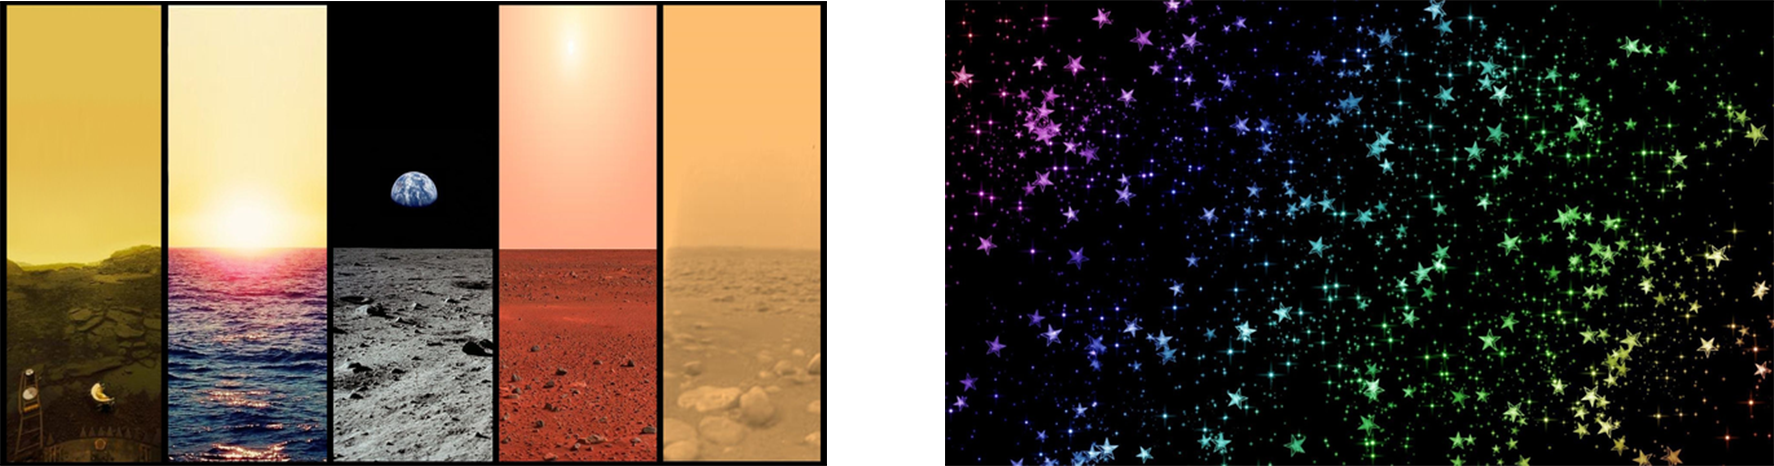
\includegraphics[width=0.7\columnwidth]{lowest_highest}
\caption{{\label{fig:minmaximg}
Image with the lowest loss value; \emph{Right}:
    Image with the highest loss value%
}}
\end{center}
\end{figure}

\chapter{Discussion}
\label{chap:discussion}

In this chapter, the results of the experiments are discussed with
regards to accuracy, frequency, and future improvements. Afterward, in
the General Discussion, the research questions are addressed and
discussed.

The comparison between sub-sampling and full sampling
(Experiment~\ref{sec:numtextons}) has shown that only a small part of
the maximum amount of samples is necessary. In fact,
$\frac{400}{640 \times 480} = 0.13\,\%$ of the maximum amount of
samples suffices to achieve cosine similarities between the texton
histograms larger than $99\,\%$. This set the stage for large
speed-ups during live operation. Additionally, the technique allows
for further speed-ups depending on the processing power of the
platform at hand.

In the real-time position estimation experiment
(Experiment~\ref{sec:experiment-real}), the initial mean error
was rather large: 130\,cm in $x$-direction and 90\,cm in
$y$-direction. A more in-depth analysis revealed that the estimates of
the particle filter were lacking behind the position estimates of the
motion tracking system. This was due to the simple motion model of the
particle filter that was based on Gaussian noise only. By shifting the
estimates of the particle filter by six frames, that is approx. 0.46
seconds at a frequency of 13\,Hz, the error could be reduced to 46\,cm
in $x$-direction and 54\,cm in $y$-direction. This lag can be
addressed by to strategies: (i) slower speed during flight, (ii) a
better or more flexible motion model.

The triggered landing (Experiment~\ref{sec:triggered}) showed a high
accuracy. While most landings were triggered inside the landing zone,
two out of the six landings were outliers. However, their distance to
the landing area were rather small, with an average distance of
16\,cm. A comparison without the safety criterion, showed, that the
criterion can have advantages.

The evaluation of different maps using the synthetic data showed high
differences between the evaluated images. The range of losses from
0.24 to 0.99 underlines the varying suitability of different maps for
the proposed algorithm.
% To visually evaluate the map evaluation technique, a simple map was
% constructed with two repeating tiles.
The
image with the minimum and the one with the maximum loss value based
on their color histogram are shown in Figure~\ref{fig:minmaximg}. The
different patterns of the images are clearly visible: while the image
with the minimum value fulfills the desired properties---closeby areas
have similar color values, distant areas are dissimilar, the image
with the maximum loss is mainly black resulting in similar histograms
all over the place and leading to high loss values. This initial
evidence can be taken to test the predictive power of the evaluation
algorithm for texton histograms.

\section{General Discussion}
\label{sec:generaldiscussion}

In this chapter, the results will be discussed regarding error
statistics, execution frequency, robustness, and scalability. To begin
with, we recapitulate the research questions:

\begin{itemize}
\item R1: Can accurate 2D positions be estimated in real-time, using a
  machine learning-based approach on a limited processor in a
  modifiable indoor environment?
\item R2: Is accurate real-world localization regression or classification
  possible when the training data comprises synthetic data only?
\item R3: Can we predict the goodness of a given map for the proposed
  localization approach?
\end{itemize}

Regarding R1, the conducted experiments provide supportive evidence
that a texton-based machine learning approach is able to accomplish
real-time indoor localization. The proposed algorithm runs with as
frequency of 30\,Hz on a single board computer with limited
CPU. Shifting processing power to an offline training step and relying
on random sampling are the cornerstones for running the algorithm on
processors with limited CPU. Despite the small ratio between extracted
image patches ($s$) and the maximum amount of different image matches
($s*$), the accuracy is hardly affected, and only slightly improves
when incorporating more textons.

Regarding research question R2, the initial idea---to use the
synthetically generated images directly as training data---was not
successful and not further followed up. This might be also the reason
that only few projects have used synthetic images for real-world
phenomena. The reality gap between the synthetic data and real-world
data was huger than expected. Figure~\ref{fig:realitygap} shows an
example of two image patches, one synthetically generated, one taken
with the camera of the MAV. While the patches can be easily identified
as similar for human eyes, the texton maps, where different colors
represent different textons, are dissimilar. Blur, lighting settings,
and camera intrinsics modify low-level features of the image to a too
strong extent. A possible improvement might be to find a mapping from
histograms of synthetic images to histograms of real images, by
mapping 'synthetic textons' to 'real-world textons'.

Referring to R3, we found some initial evidence that the proposed map
evaluation generalizes to the real-world. In contrast to R2, the
generalization from the synthetic data to real-world data is of a
different nature in this case. The requirement here is that maps that
follow the ideal similarity distribution in the synthetically
generated images also follow this distribution after being recorded
with a camera. Or stated differently, for maps with a low loss value,
distant image positions should not have similar histograms using the
synthetic images nor the real-world images.

Despite the overall promising results, we noticed drawbacks of the
proposed approach during the flight tests and directions for future
research.

The accuracy---that is the difference between the estimates of the
motion tracking system and the texton-based approach--- could be
further improved by incorporating more features, for example histogram
of oriented gradients. Additional improvements could be obtained by
investigating further regression techniques, like Gaussian processes
or Bayesian networks that can inherently handle space and time.

The developed method sets the stage for numerous future research
directions and improvements. The current implementation assumes rather
constant height up to few centimeters and no yaw rotations of the
MAV. While a quadroter can move in every direction without performing
yaw movements, using the algorithm on another vehicle could require
arbitrary yaw movements. To limit the complexity of the dataset, a
``derotation'' of the incoming image could be performed to align it
with the underlying images of the dataset. While the current approach
normalizes each $5\times5$ image patch to unit mean and zero
variance---giving robustness to different lighting conditions---this
procedure could be further extended, for example by using specific
color models.

While the current map evaluation approach used existing fixed images,
it could also serve as a fitness function for an optimization
approach---for example, an evolutionary algorithm---which modifies a
given image. This could allow to find a near optimal solution for a
given regression technique and give insightful view in the underlying
structure of certain regression techniques. While the solution to a
loss value of zero or near zero might be unique and independent of the
original image, a higher loss value might change the initial image
only to a certain extent, yielding an ``improved version of the
image'', which is better suited for the proposed algorithm.

The presented software \emph{draug} generates image patches based on
drawing samples from parametric distributions only. This was motivated
by the fact that an ideal map should be independent of previous
estimates and based on single images only---ideally requiring no
filtering. In the future, the possibility to set flight routes by
setting way points above an image could be included. This would allow
to test the ability of the particle filter on synthetic flights.

\begin{figure}[h!]
\begin{center}
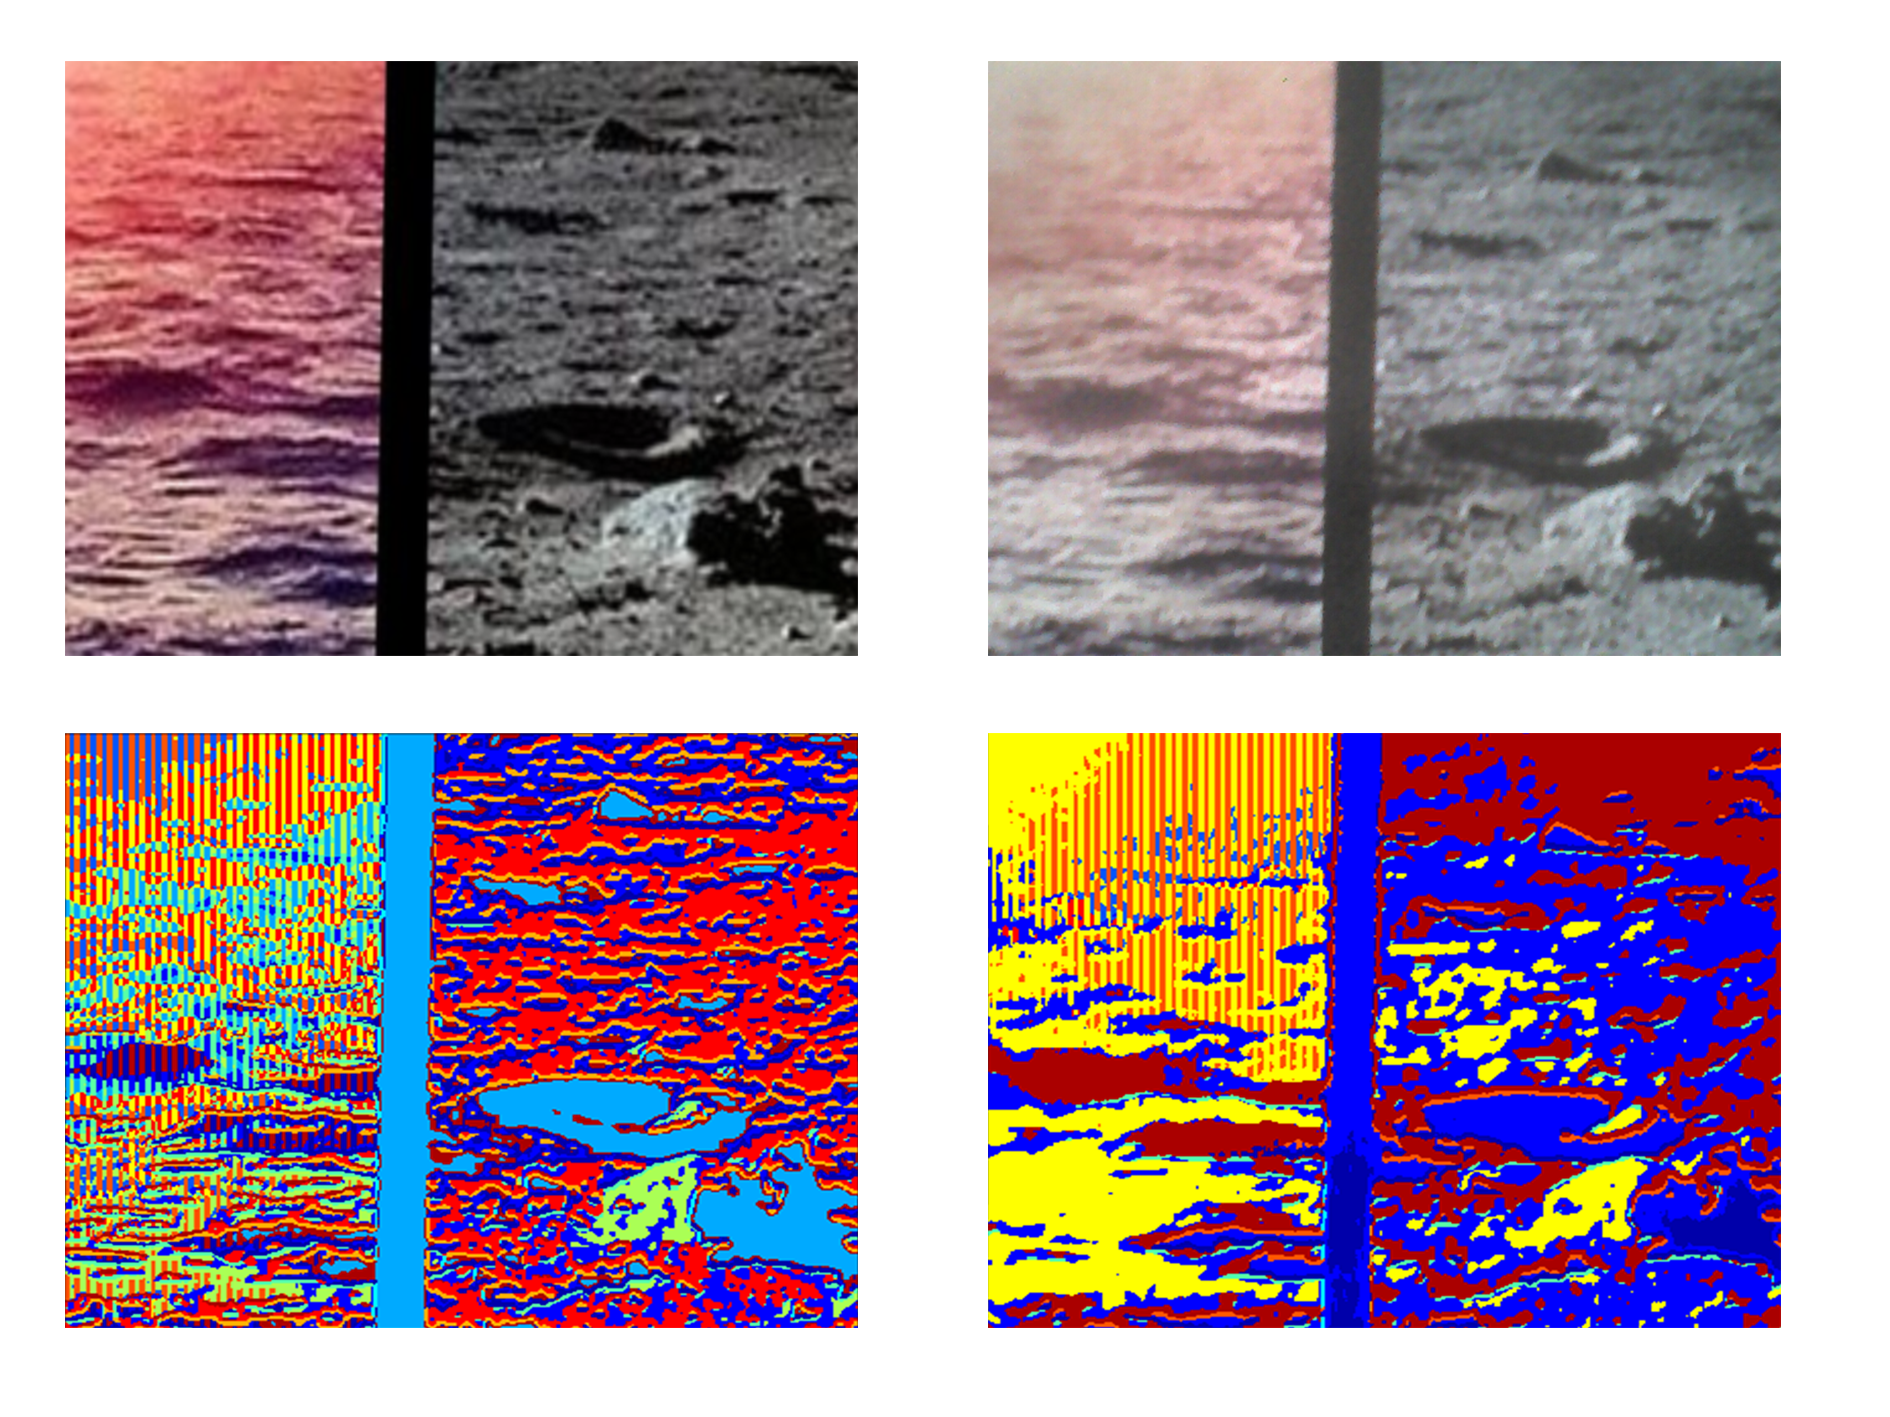
\includegraphics[width=0.448\columnwidth]{realitygap}
\caption{{\label{fig:realitygap}
Exemplifying the reality gap. \emph{Top left}: image patch generated using draug. \emph{Top
      right}: image patch taken with the MAV's camera after printing
    the patch. \emph{Below left}: texton image of the synthetic
    image. \emph{Below right}: Texton image of the real image. The
    texton images shows that corresponding regions get classified into
    different textons, resulting in different histograms. This makes
    the transfer from the synthetic data to the real world difficult.%
}}
\end{center}
\end{figure}

The shift of the processing power could be further amplified by using
a different regression technique. In the current implementation using
$k$-NN regression, larger training data sets are penalized due to a
greater prediction time. However, the choice of a different regression
technique is not as straightforward as it might seem. The technique
should be able to output multiple predictions, since certain map
regions might be ambiguous.

The presented approach is a vision-only approach. This makes it robust
to external disruptions such as magnetic fields and reduces the amount
of points of failure. Additionally, the approach can be used on
different devices, such as handheld cameras. Still, future
developments could incorporate data from the inertial measurement unit
(IMU) in the particle filter's motion model.

Additionally, the time complexity of the algorithm can be further
reduced with the aim of running the algorithm on fly-sized
MAVs. Depending on the target platform, parallelization or threading
could be used on multi-core systems to simultaneously compute texton
histograms, make predictions and run the particle filter.

% Currently, the computationally most complex part is the XXX.